% Chapter Template

\chapter{CARACTERIZACION DE UN BMG BAJO DIFERENTES MODOS DE CARGA Y TEMPERATURAS} % Main chapter title

\label{C3} % Change X to a consecutive number; for referencing this chapter elsewhere, use \ref{ChapterX}

\lhead{Capítulo 3. \emph{CARACTERIZACION DE UN BMG BAJO DIFERENTES MODOS DE CARGA Y TEMPERATURAS}} % Change X to a consecutive number; this is for the header on each page - perhaps a shortened title

%----------------------------------------------------------------------------------------
%	SECTION 1
%----------------------------------------------------------------------------------------
%\section{Abstract}

%Amorphous metals, i.e. without defined crystal structure; are increasingly used in modern life, showing great potential as advanced engineering materials, due to some of its characteristic properties such as high hardness and moldability, high resilience, high mechanical strength and high wear resistance, among others. All these properties allow obtaining parts with complex shapes and high strength, which increases their chances for industrial application. However, many details of the mechanical behavior are still unknown, and the currently used models and theories are far from predictive.
%One of the possibilities to determine constitutive parameters, and thus study the response of these materials, is by using atomistic calculations. In this paper we present results obtained with molecular dynamics (MD) simulations, of an amorphous metal (CuZr). In particular, constitutive parameters such as elasticity modulus, are determined for samples at different temperatures and subjected to both tension and compression. The results obtained are relevant for understanding the mechanical behavior of the material, such as stress-strain and temperature-strain relationships. Additionally, it is possible to observe, under uniaxial tension, the nucleation and growth of a void due to high stress and strain rate values.

\section{Introducción}
%Los materiales sólidos sin una estructura ordenada, es decir, amorfos, son llamados generalmente "vidrios". Algunos casos particulares de gran interés científico y tecnológico son los vidrios metálicos, que son aleaciones metálicas con propiedades mecánicas que sobrepasan en prestaciones a las aleaciones cristalinas más comunes (\cite{luborsky83}, \cite{greer95}). Se sabe que los metales forman fácilmente cristales cuando son enfriados (\cite{callister95}, \cite{smith96}). Sin embargo, usando una velocidad de enfriamiento suficientemente elevada y controlando la composición de la aleación, es posible obtener estructuras amorfas (\cite{liebermann93}), con la elasticidad de los polímeros y la resistencia de los metales (\cite{telford04}), teniendo también alta resistencia y moldeabilidad. Estas propiedades en su conjunto hacen posible la creación de partes de forma compleja y de alta resistencia, lo que además incrementa sus posibilidades de ser utilizados en aplicaciones industriales. Gracias a las propiedades citadas, estos materiales han sido de mucho interés como materiales estructurales en años recientes (\cite{chen74}, \cite{lowhaphandu99}, \cite{inoue00}, \cite{wang04}, \cite{ashby06}, \cite{zhang07}, \cite{schuh07}), incluyendo, por ejemplo, metales amorfos estructurales (\cite{lu04}), materiales biomédicos (\cite{zberg09}) o hasta incluso materiales aeroespaciales (\cite{peker93}), por nombrar algunos.

%Solid materials without an ordered structure, i.e. amorphous, are generally called "glasses". Particular cases of great scientific and technological interest are metallic glasses, which are metallic alloys with mechanical properties that outperform the most common crystalline alloys (\cite{luborsky83}, \cite{greer95}). It is known that metals easily form crystals when cooled (\cite{callister95}, \cite{smith96}). However, using a sufficiently fast cooling rate and controlling the composition of the alloy it is possible to obtain amorphous structures (\cite{liebermann93}), with the elasticity of polymers and the resistance of metals (\cite{telford04}), also having high strength and moldability. All these properties enable the creation of parts with complex shapes and high resistance, which further increases their chances of industrial applications. Thanks to the above properties, these materials have received great interest as structural materials in recent years (\cite{chen74}, \cite{lowhaphandu99}, \cite{inoue00}, \cite{wang04}, \cite{ashby06}, \cite{zhang07}, \cite{schuh07}), including, for example, amorphous structural steels (\cite{lu04}), biomedical materials (\cite{zberg09}) or even aerospace materials (\cite{peker93}), to name a few.

Los vidrios metálicos son clasificados en general como vidrios metálicos convencionales o vidrios metálicos masivos (BMG) (\cite{wang04}, \cite{miller07}). Los BMG han sido recientemente empleados como fase matriz en materiales compuestos, mejorando varias de las propiedades originales de la fase dispersa como las propiedades mecánicas, magnéticas, etc. (\cite{telford04}, \cite{lu11}). En el caso particular de vidrios metálicos bajo deformación plástica, con la aparición de bandas de corte, de costumbre se abarca el problema con un enfoque en el comportamiento a nivel nano (\cite{ogata06}, \cite{guan10}), o mediante una aproximación usando mecánica del continuo (\cite{malvern69}).

%Metallic glasses can generally be classified as conventional metallic glasses or bulk metallic glasses (BMG) (\cite{wang04}, \cite{miller07}). BMG have recently been employed as matrix phase in composite materials, thus improving the various original properties of the dispersed phase such as mechanical, magnetic properties, etc. (\cite{telford04}, \cite{lu11}). In the particular case of metallic glasses under plastic strain, with the appearance of shear bands, it is customary to address the problem through a focus on nanoscale behavior (\cite{ogata06}, \cite{guan10}), or through an approach using continuum mechanics (\cite{malvern69}).

%Las simulaciones de dinámica molecular (MD) son usadas frecuentemente para estudiar propiedades a escala nano (\cite{allen87}). Las simulaciones de MD son una técnica muy poderosa que permite resolver, usando mecánica clásica, problemas con muchos cuerpos, dada una interacción entre átomos. Una ventaja de MD es que la deformación, el esfuerzo, la temperatura, la velocidad, etc. son todas conocidas en detalle (\cite{allen87}). Con esta información un gran número de fenómenos pueden estudiarse, como cambios de fase, transferencia de calor, creación y movimiento de dislocaciones, defectos, etc.. MD es una herramienta muy versátil para el estudio de las propiedades de materiales, y hasta ha sido utilizada para predecir el comportamiento mecánico de materiales previamente a los experimentos, como en el caso de maclas de aluminio (\cite{chen03}). Las simulaciones de MD reproducen el movimiento atómico y por lo tanto emplean pasos de tiempo de 1 fs (\cite{allen87}). Si modelamos una muestra hasta 10\% de deformación durante 1 millón de pasos de 1 fs, la velocidad de deformación será de $10^8$/s, que es adecuada para simular la deformación bajo láser de alta potencia, pero está lejos de serla para la mayoría de ensayos mecánicos en laboratorios. Como resultado, la extrapolación de resultados a bajas velocidades de deformación, debe realizarse cuidadosamente (\cite{bringa05}).

%Molecular dynamics (MD) simulations are often used to study nanoscale properties (\cite{allen87}). MD simulations are a very powerful technique that allows solving, using classical mechanics, problems with many bodies, given an interaction between atoms. One advantage of MD is that strain, stress, temperature, speed, etc. are all known in detail (\cite{allen87}). From this information large number of phenomena can be studied, such as phase changes, heat transfer, creation and movement of dislocations, defects, etc.. MD is a very versatile tool for studying the properties of materials, and has even been used to predict mechanical behavior of materials prior to  experiments, as in the case of aluminum twinned nanocrystals (\cite{chen03}). MD simulations reproduce the atomic motion and therefore employ time steps of 1 fs (\cite{allen87}). If modeling a sample up to 10\% strain during 1 million steps of 1 fs, the strain rate will be 108 /s, which is suitable for simulating deformation by high power lasers, but far from the majority of mechanical tests in laboratories. As a result, extrapolation to low strain rates has to be done carefully (\cite{bringa05}).

%Existen múltiples simulaciones de MD de metales amorfos. Las simulaciones de vidrios metálicos en particular se incrementaron por la presencia de potenciales de interacción adecuados para el sistema CuZr (\cite{ogata06}, \cite{arman10}, \cite{guan10}). En esta sección presentamos simulaciones de nivel atómico de un vidrio metálico CuZr sujeto a tracción y compresión, y analizamos sus respuestas como función de la temperatura.

%There are numerous molecular dynamics simulations of amorphous materials. The simulations of metallic glasses in particular have increased due to the presence of suitable interaction potentials for the CuZr system (\cite{ogata06}, \cite{arman10}, \cite{guan10}). In this paper we present atomic-scale simulations of CuZr metallic glasses subjected to tension and compression, and analyze their response as a function of their temperature.

En esta sección presentamos simulaciones de nivel atómico (utilizando dinámica molecular) de un vidrio metálico CuZr sujeto a tracción y compresión, y analizamos sus respuestas como función de la temperatura.

\section{Detalles de las simulaciones}

%In this paper, simulations were carried out using the LAMMPS software (\cite{plimpton95}), which is free and open source, has an excellent manual, and is computationally efficient in the simulation of systems with large numbers of atoms.

La muestra Cu$_{46}$Zr$_{54}$ usada es prismática, con un total de alrededor de 160k átomos, creada con una velocidad de enfriamiento de $10^12$ K/s, y ya ha sido descrita por \cite{arman10}. En su trabajo, se estudiaron los efectos de ondas de choque en BMGs. La temperatura experimental de transición vitrea (Tg) de este vidrio metálico es 696 K, y su módulo de cizalla experimental (G) es 30 GPa (\cite{johnson05}). Se incluye un caso de simulación a 900 K, sobre Tg, para ver si el comportamiento mecánico es significativamente diferente. Para describir las interacciones entre átomos, un potencial de método de átomo embebido (EAM) (\cite{daw84}) fue adoptado, que ya ha sido usado en otros estudios sobre BMGs (\cite{shimizu07}, \cite{cao09}, \cite{cheng08}, \cite{arman10}, \cite{cheng11}, \cite{wang12}).

%The Cu$_{46}$Zr$_{54}$ sample used is prismatic, with a total of about 160k atoms, obtained with a quenching rate of 1012 K/s, and it has already been described by \cite{arman10}, in their study effect of shock waves in BMGs was studied. The experimental glass transition temperature (Tg) of this metallic glass is 696 K, and the experimental shear modulus (G) is 30 GPa (\cite{johnson05}). We include a simulation case at T=900 K, above Tg, to see if the mechanical behavior is significantly different. To describe the interactions between atoms, an embedded atom method (EAM) potential (\cite{daw84}) is adopted, which has already been used in other BMGs studies (\cite{shimizu07}, \cite{cao09}, \cite{cheng08}, \cite{arman10}, \cite{cheng11}, \cite{wang12}).

Usamos condiciones de borde periódicas en 3D, válidas para altas velocidades de deformación (\cite{bringa05}). Todas las coordenadas atómicas son escaladas a cada paso, de acuerdo con la velocidad de deformación deseada, que en este caso es de $10^9$ /s. Antes de iniciar las deformaciones mecánicas, se realiza primero una minimización de energía usando el gradiente conjugado, y luego usamos condiciones de presión cero y temperatura constante para equilibrar la muestra a la temperatura buscada T. La Tabla \ref{C3:tb:initprops} presenta los volúmenes y densidades iniciales para los diferentes casos.

%We use 3D periodic boundary conditions, suitable for high strain rates (\cite{bringa05}). All atomic coordinates are scaled every step, according to the desired strain rate, which in this case was 10$^{9}$ /s. Before starting mechanical strain simulations, we first perform energy minimization using conjugate gradient, and then use zero-pressure conditions and constant temperature to equilibrate the sample to the desired temperature T. Table 1 lists the volumes and initial sample densities for the different cases.

\begin{table}[htp]
\caption[Volúmenes y densidades iniciales.]{Volúmenes y densidades iniciales a diferentes temperaturas simuladas.}
\begin{center}
\begin{tabular}{*{3}{c}}
Temperatura [$K$] & Volumen [$nm^{3}$] & Densidad [$\frac{g}{cm^{3}}]$ \\
10K & 2909.15 & 7.1705 \\
300K & 2931.93 & 7.1147 \\
600K & 2959.54 & 7.0484 \\
900K & 2992.30 & 6.9712
\end{tabular}
\end{center}
\label{C3:tb:initprops}
\end{table}

\section{Resultados}

En el texto que continúa, presentamos resultados para tensión exclusivamente uniaxial, la cual es apropiada para la comparación con resultados de experimentos a una velocidad de deformación muy elevada, en donde las deformaciones laterales pueden despreciarse. La Figura \ref{C3:fg:sStrain} \subref{C3:fg:sStrainTen} muestra nuestros resultados para tensión de von Mises versus deformación a todas las temperaturas simuladas. Luego de la deformación puramente elástica que ocurre hasta alrededor de 2\% de deformación, existe un decremento en la tensión de von Mises, lo que sugiere la presencia de plasticidad. Además, dadas la grandes velocidades de deformación y las grandes deformaciones, se nuclea un poro en la muestra bajo tracción, como vemos en la Figura \ref{C3:fg:voidSeq}, que lleva a grandes fluctuaciones de la tensión luego de aproximadamente 15\% de deformación.

%Below we present results for purely uniaxial strain, which is appropriate for the comparison with results of experiments at very high strain rates, where lateral strains can be neglected.
%Figure 1 (a) shows our results for von Mises stress versus strain at all the simulated temperatures. After the purely elastic deformation that occurs up to about 2\% strain, there is a decrease in von Mises tension, suggestive of plasticity. In addition, due to the high strain rates and large stress, there is a void nucleation in the sample under tension, as shown in Figure 2, which leads to large stress fluctuations after about 15\% strain.

\begin{figure}[htp]
\centering
\subfloat[Tracción]{
	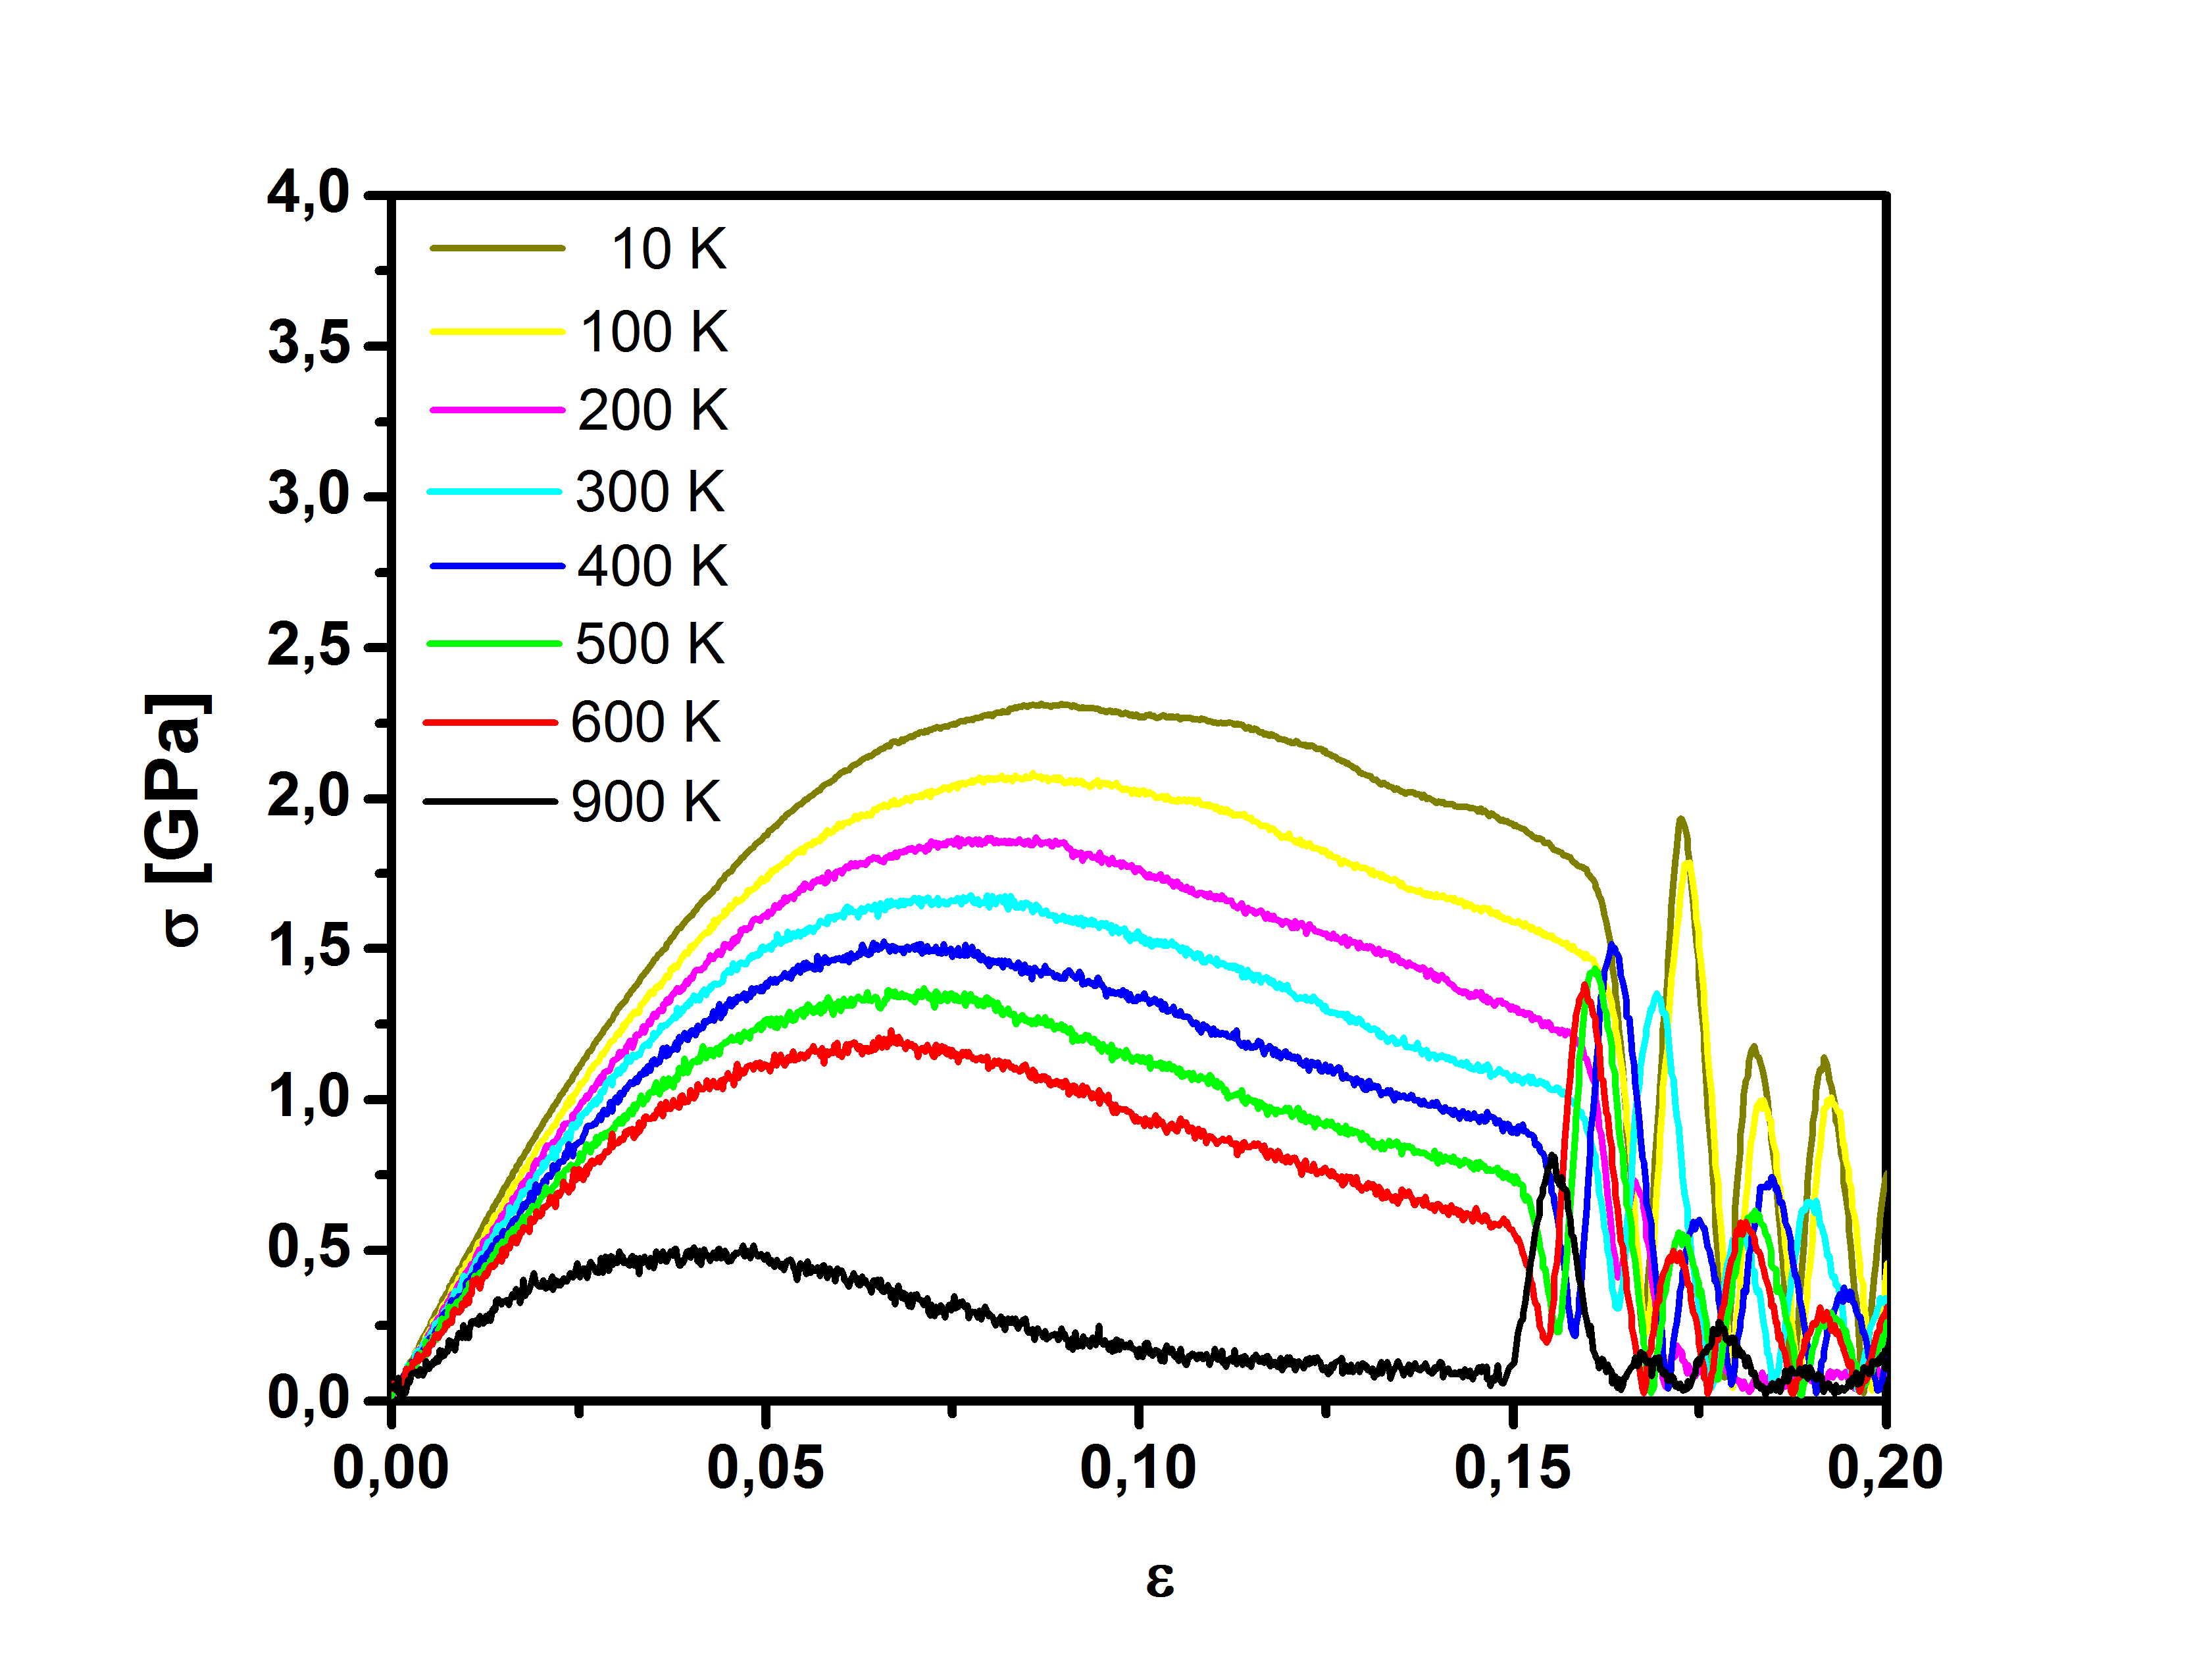
\includegraphics[width=8cm]{Cap_3/stress_strain_TEN.png}
	\label{C3:fg:sStrainTen}}
\subfloat[Compresión]{
	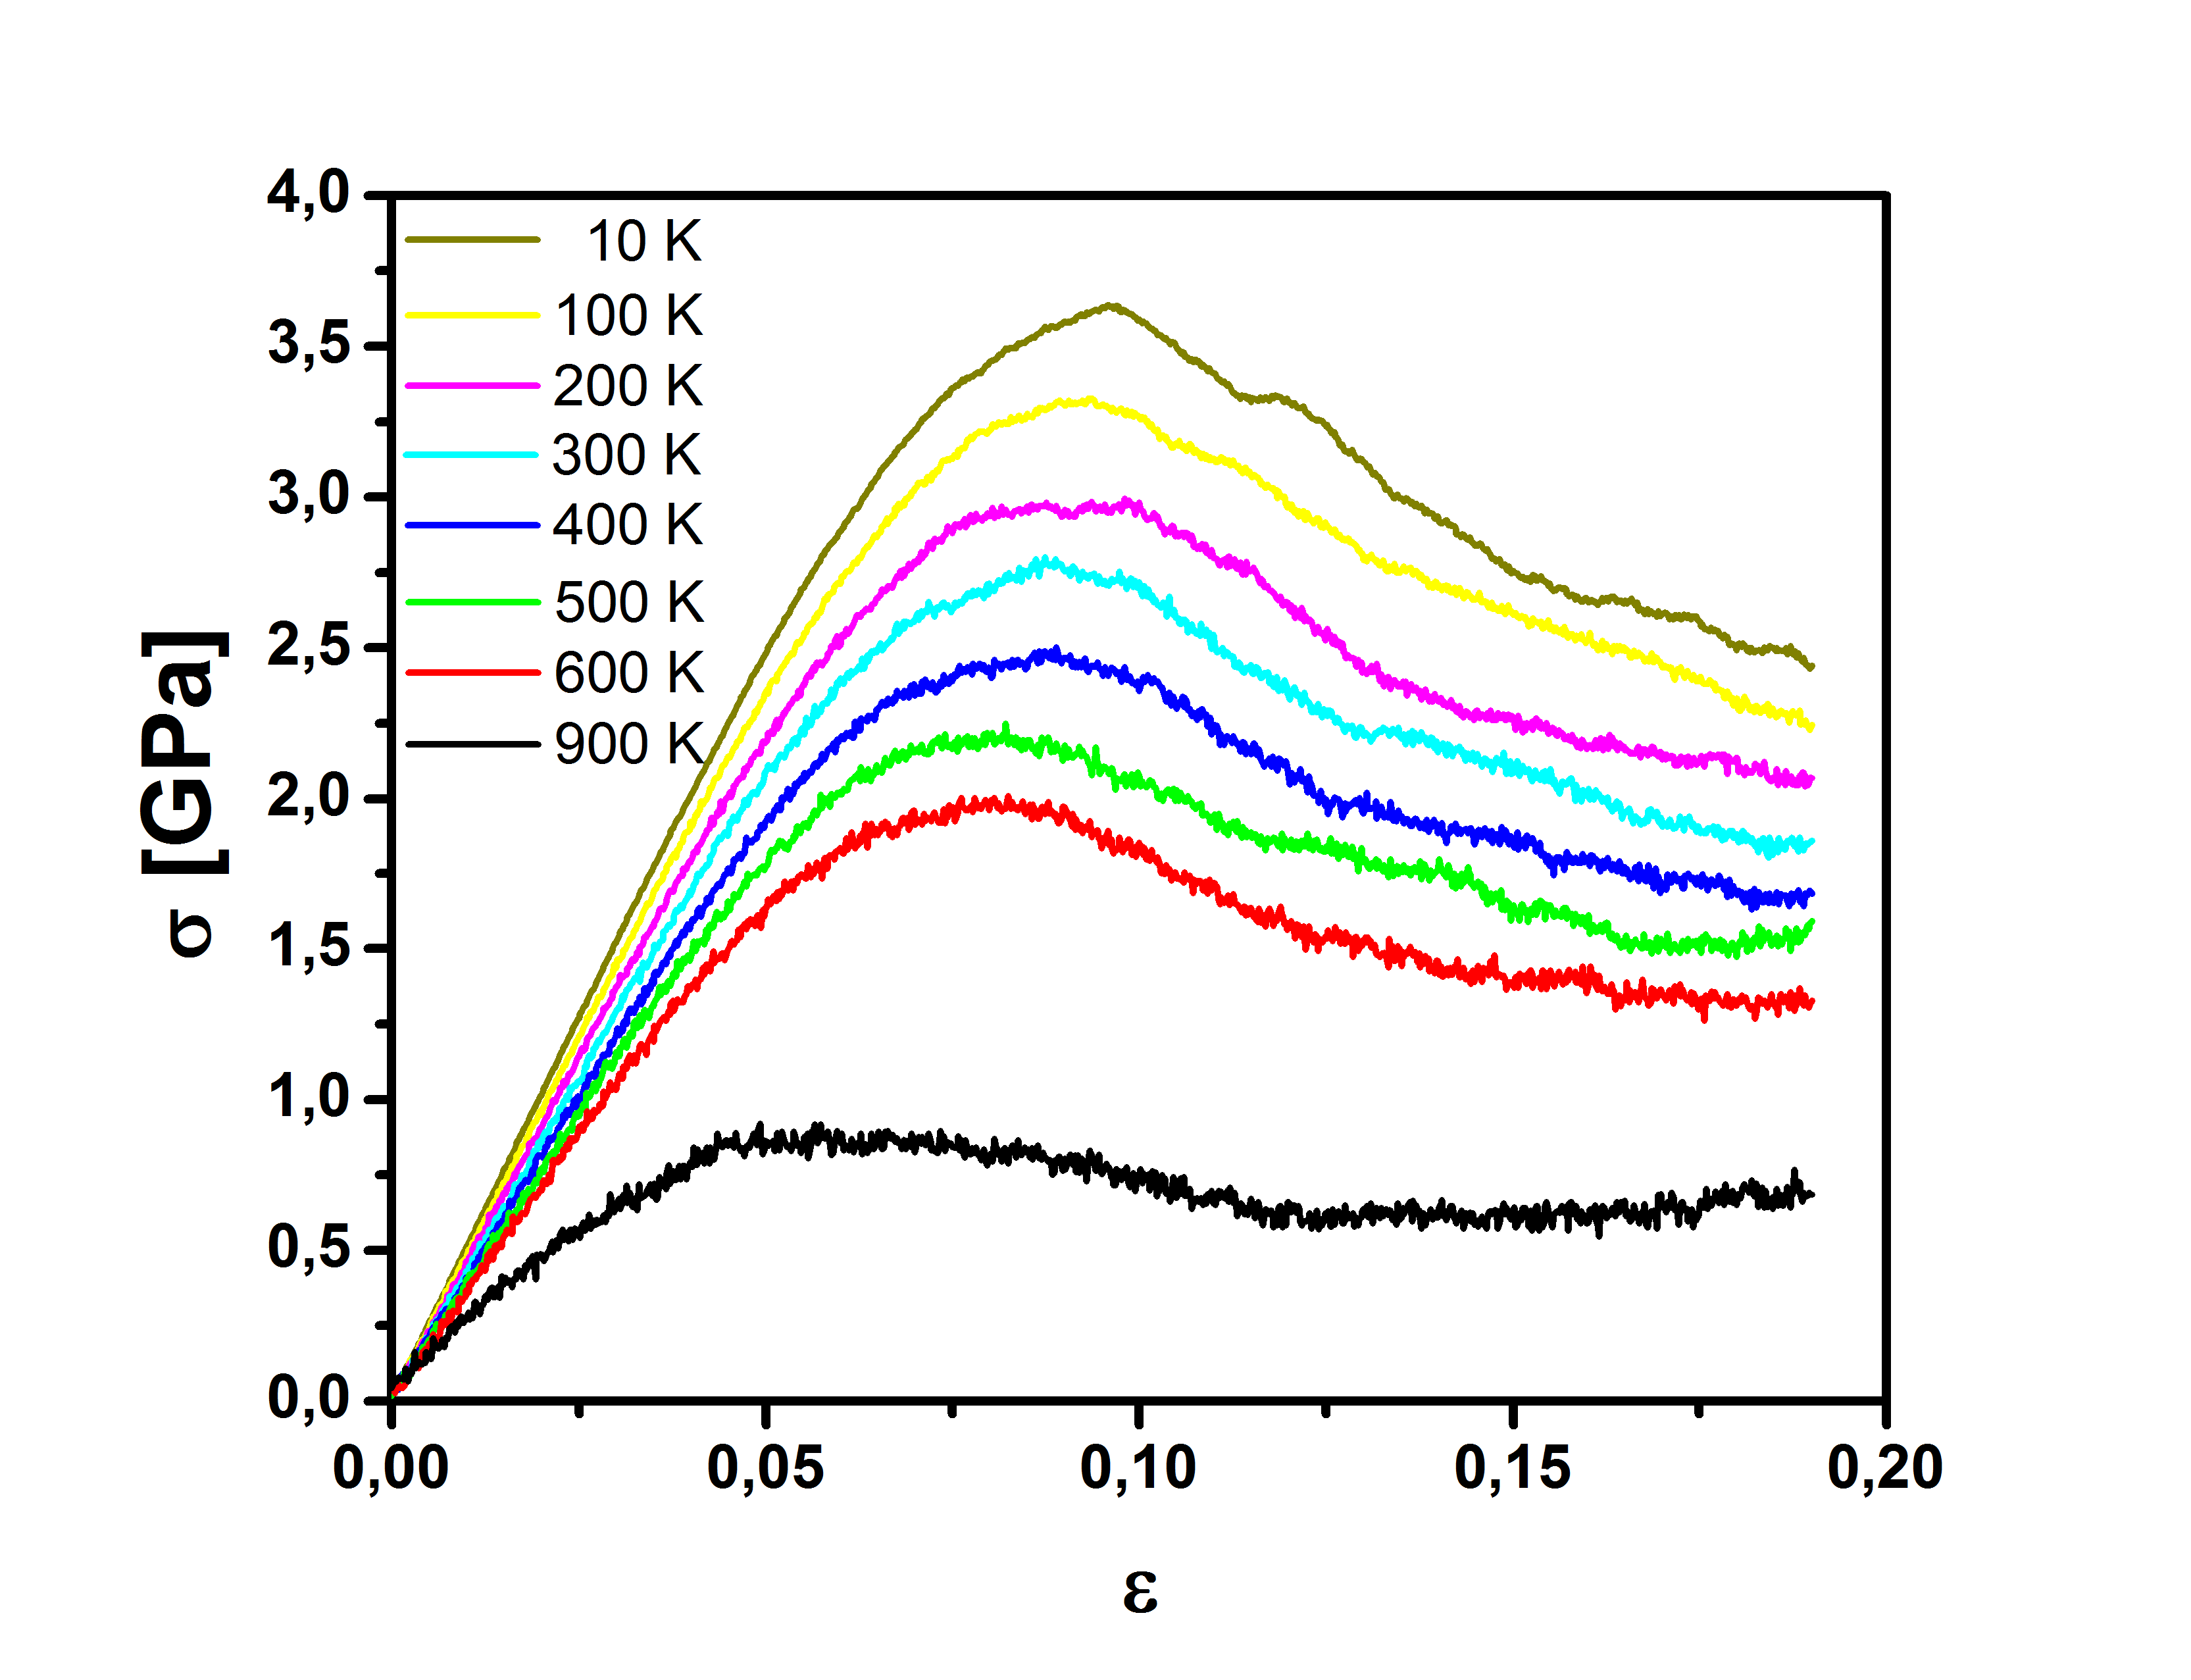
\includegraphics[width=8cm]{Cap_3/stress_strain_COMP.png}
	\label{C3:fg:sStrainComp}}
\caption[Curvas de esfuerzo-deformación a diferentes temperaturas.]{Curvas de esfuerzo-deformación a diferentes temperaturas. Bajo tracción existen grandes fluctuaciones del esfuerzo que comienzan cuando se nuclea un poro a aproximadamente 15\% de deformación.}
\label{C3:fg:sStrain}
\end{figure}

\begin{figure}[htp]
\centering
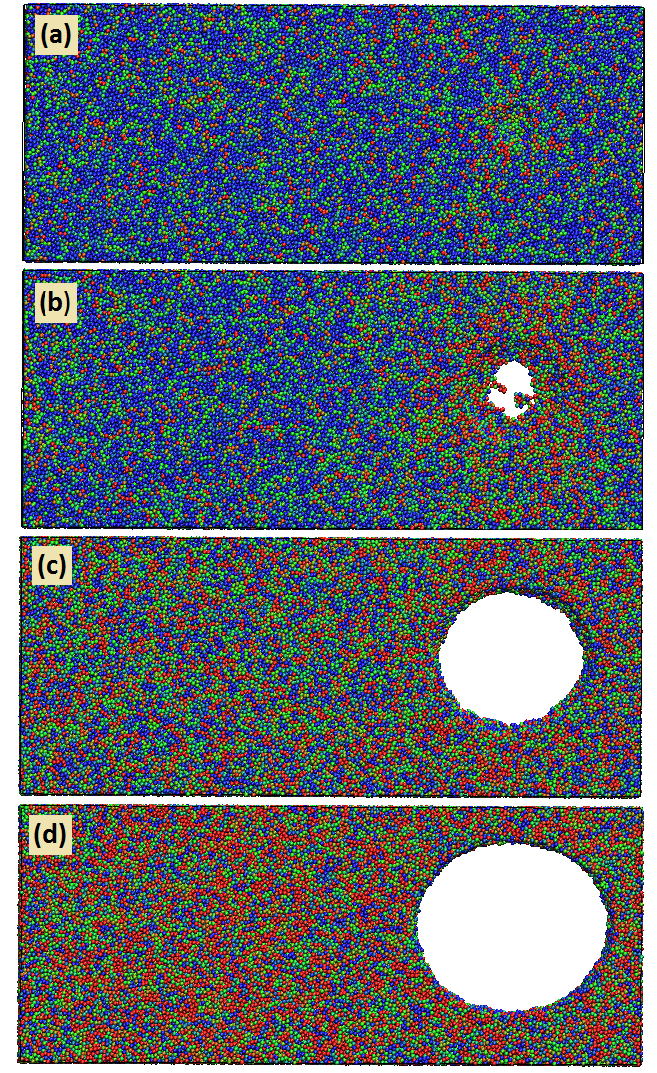
\includegraphics[width=10cm]{Cap_3/void_sequence.png}
\caption[Nucleación de un poro bajo tracción a 900 K.]{Nucleación de un poro bajo tracción a 900 K. (a) $\epsilon$ = 0.137 (b) $\epsilon$ = 0.141 (c) $\epsilon$ = 0.145 (d) $\epsilon$ =0.149. Los colores representan la tensión de von Mises, rojo siendo alta tensión y azul baja tensión. Una nucleación similar es observada a temperaturas más bajas.}
\label{C3:fg:voidSeq}
\end{figure}

Calculamos las propiedades mecánicas y proponemos la siguiente forma funcional como aproximación del comportamiento térmico:

%We calculate mechanical properties, and propose the following simple functional form as an approximation for the thermal behavior:

\begin{eqnarray}
y = A_{1}\cdot \mathrm{e}^{\frac{-T}{T_{0}}}
\label{C3:eq:thermalFit}
\end{eqnarray}

donde $A_{1}$ y $T_{0}$ son parámetros. Esta forma funcional es frecuentemente usada para fenómenos activados termicamente. En las Tablas \ref{C3:tb:initPropsTen} y \ref{C3:tb:initPropsComp} presentamos los valores para los coeficientes de la Ecuación \ref{C3:eq:thermalFit} obtenidos de las curvas mostradas en las Figuras \ref{C3:fg:youngVsT}-\ref{C3:fg:peakVMises1218VsT}. Puede verse que las regresiones son razonables. El coeficiente de correlación ($R^2$) es mayor a 0.9 en todos los casos, haciendo razonable nuestra aproximación funcional simple. Por supuesto, un estudio más detallado incluyendo muchos más valores de temperatura es necesario para verdaderamente poner a prueba las aproximaciones.
	
%where $A_{1}$ and $T_{0}$ are parameters. This functional form is often used for thermally activated phenomena. In Tables 2-3 we present the values for the coefficients of equation (1) obtained from the curves shown in Figures 3-6. It can be seen that the fits are reasonable. The correlation coefficient (R2) is greater than 0.9 in all cases, thus making our simple functional fit reasonable. Of course, further studies including many more temperature values are needed to truly test the fits. 

\begin{table}[htp]
\caption[Coeficientes de la regresión para tracción.]{Coeficientes de la regresión para tracción.}
\begin{center}
\begin{tabular}{*{4}{c}}
Tracción & Parámetros & Valor & $R^{2}$ \\
Peak von Mises stress & A$_{1}$ & 2.312 $\pm$ 0.055 & 0.989 \\
 & T$_{0}$ & 1059.6 $\pm$ 68.8 & \\
von Mises stress ($\epsilon$=0.12) & A$_{1}$ & 2.23 $\pm$ 0.22 & 0.935 \\
 & T$_{0}$ & 509.4 $\pm$ 101.7 & \\
Young Modulus & A$_{1}$ & 51.3 $\pm$ 2.6 & 0.928 \\
 & T$_{0}$ & 1419.5 $\pm$ 239.0 & \\
Yield Stress & A & 0.0604 $\pm$ 0.004 & 0.952 \\
 & B & -0.041 $\pm$ 0.005 & 
\end{tabular}
\end{center}
\label{C3:tb:initPropsTen}
\end{table}

\begin{table}[htp]
\caption[Coeficientes de la regresión para compresión.]{Coeficientes de la regresión para compresión.}
\begin{center}
\begin{tabular}{*{4}{c}}
Compresión & Parámetros & Valor & $R^{2}$ \\
Peak von Mises stress & A$_{1}$ & 3.77 $\pm$ 0.23 & 0.931 \\
 & T$_{0}$ & 804.3 $\pm$ 144.2 & \\
von Mises stress ($\epsilon$=0.18) & A$_{1}$ & 2.58 $\pm$ 0.22 & 0.915 \\
 & T$_{0}$ & 863.6 $\pm$ 166.6 & \\
Young Modulus & A$_{1}$ & 52.14 $\pm$ 1.61 & 0.972 \\
 & T$_{0}$ & 1437.7 $\pm$ 146.8 & \\
Yield Stress & A & 0.123 $\pm$ 0.01 & 0.930 \\
 & B & -0.081 $\pm$ 0.013 & 
\end{tabular}
\end{center}
\label{C3:tb:initPropsComp}
\end{table}

Como es de esperarse, el módulo de elasticidad, la tensión máxima de von Mises y la tensión de fluencia, todos decrecen con el aumento de la temperatura. Obtenemos un comportamiento suave incluso cuando T supera a Tg, como puede verse en las Figuras \ref{C3:fg:youngVsT}-\ref{C3:fg:peakVMises1218VsT}.

%As expected, the elastic modulus, peak von Mises stress and yield stress, all decrease with increasing temperature. We obtained a smooth behavior even when T is above Tg, as seen in Figures 3-6.

\begin{figure}[htp]
\centering
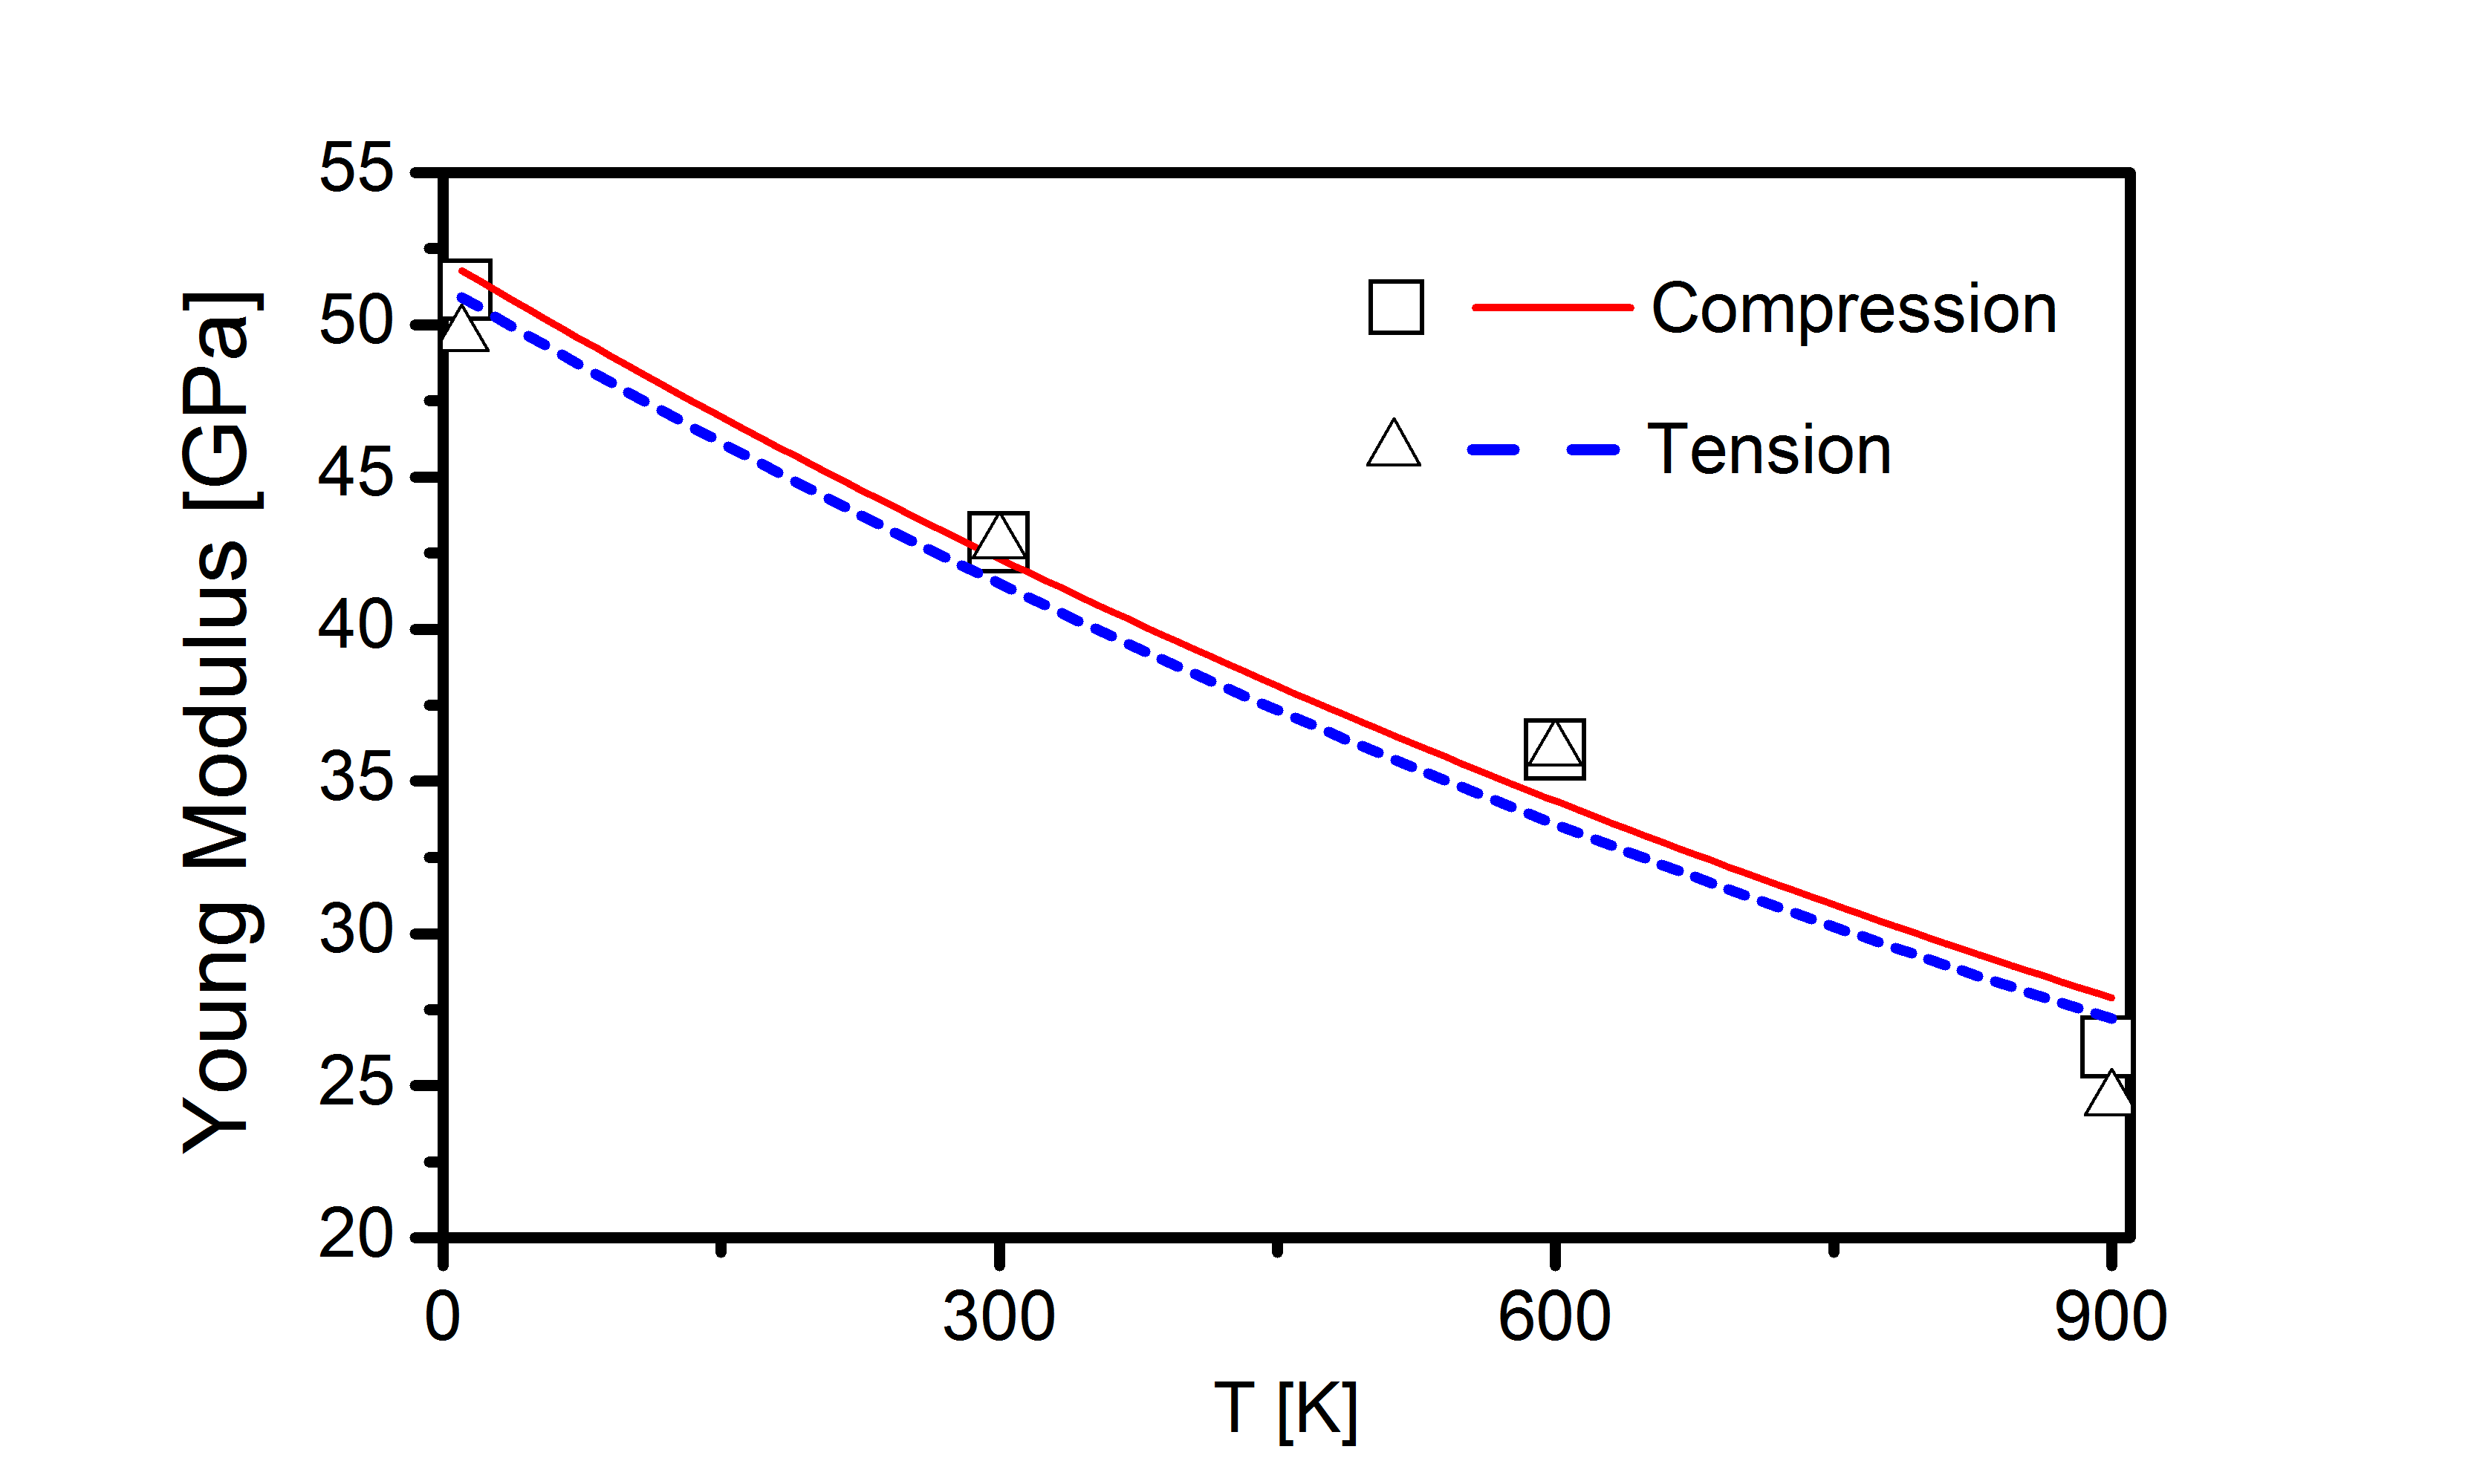
\includegraphics[width=10cm]{Cap_3/FitYoungBoth.png}
\caption[Fit módulo de Young-temperatura.]{Fit módulo de Young-temperatura.}
\label{C3:fg:youngVsT}
\end{figure}

\begin{figure}[htp]
\centering
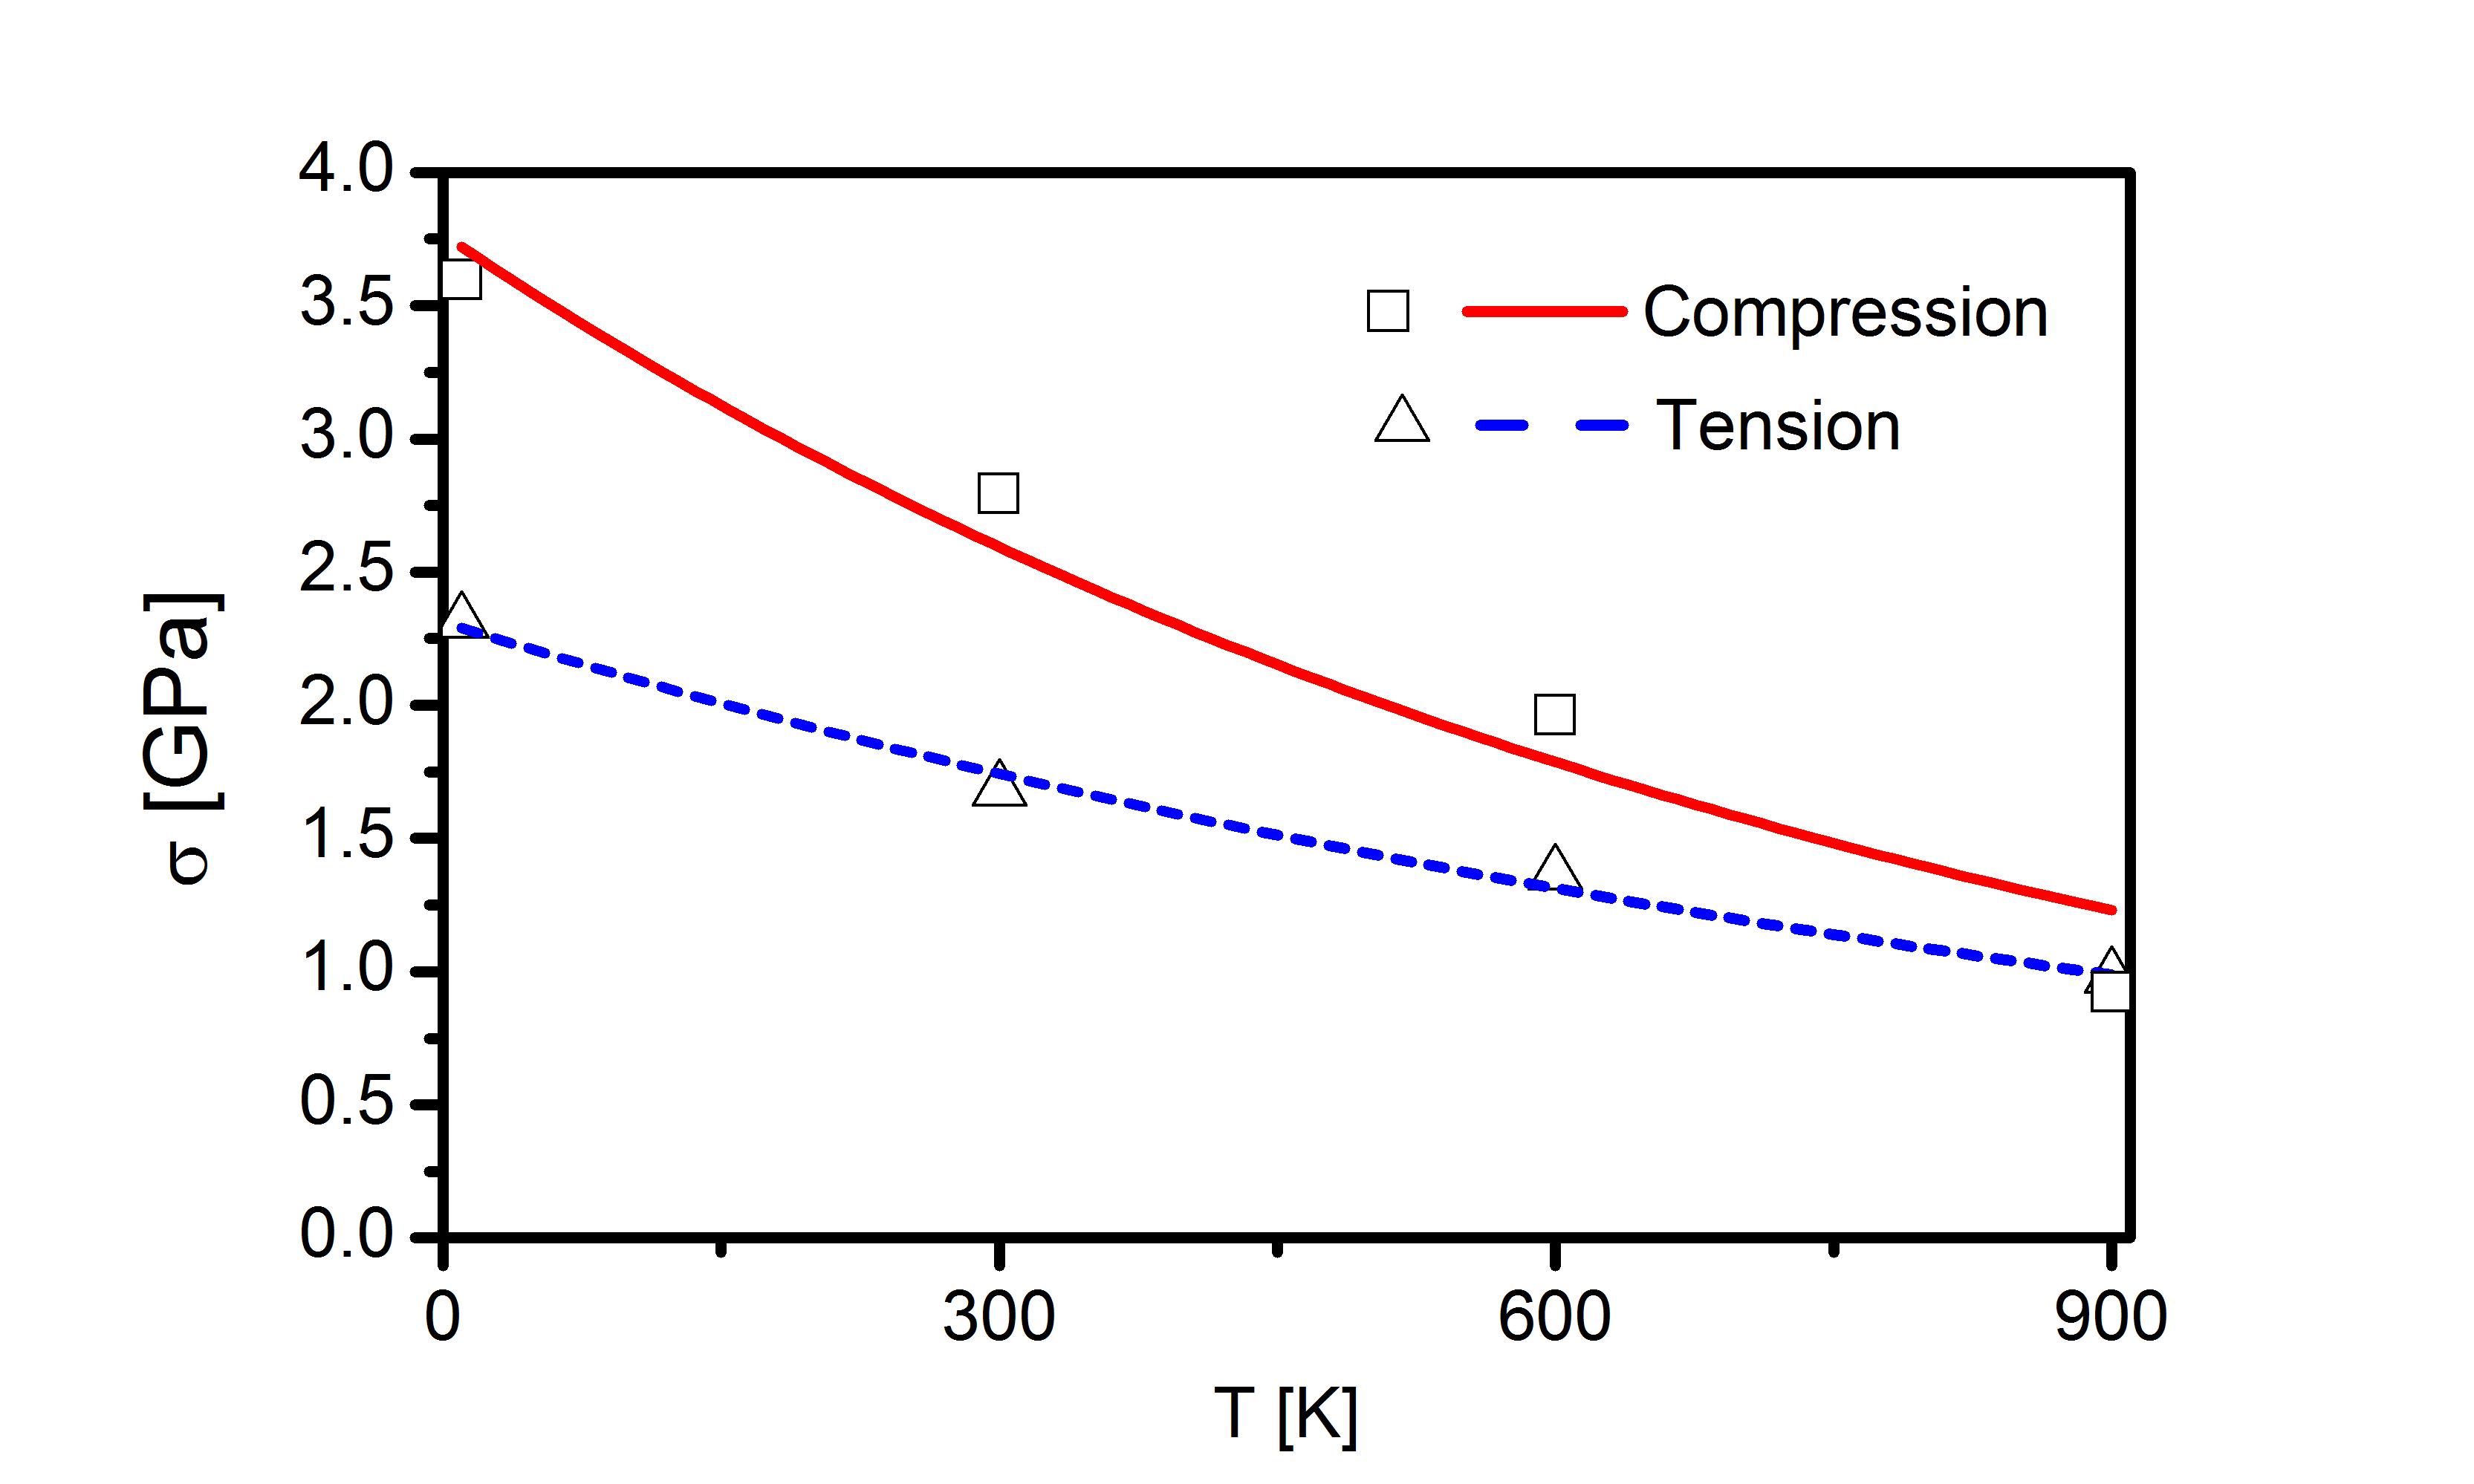
\includegraphics[width=10cm]{Cap_3/FitPeakBoth.png}
\caption[Fit tension de von Mises máxima-temperatura.]{Fit tension de von Mises máxima-temperatura.}
\label{C3:fg:peakVMisesVsT}
\end{figure}

\begin{figure}[htp]
\centering
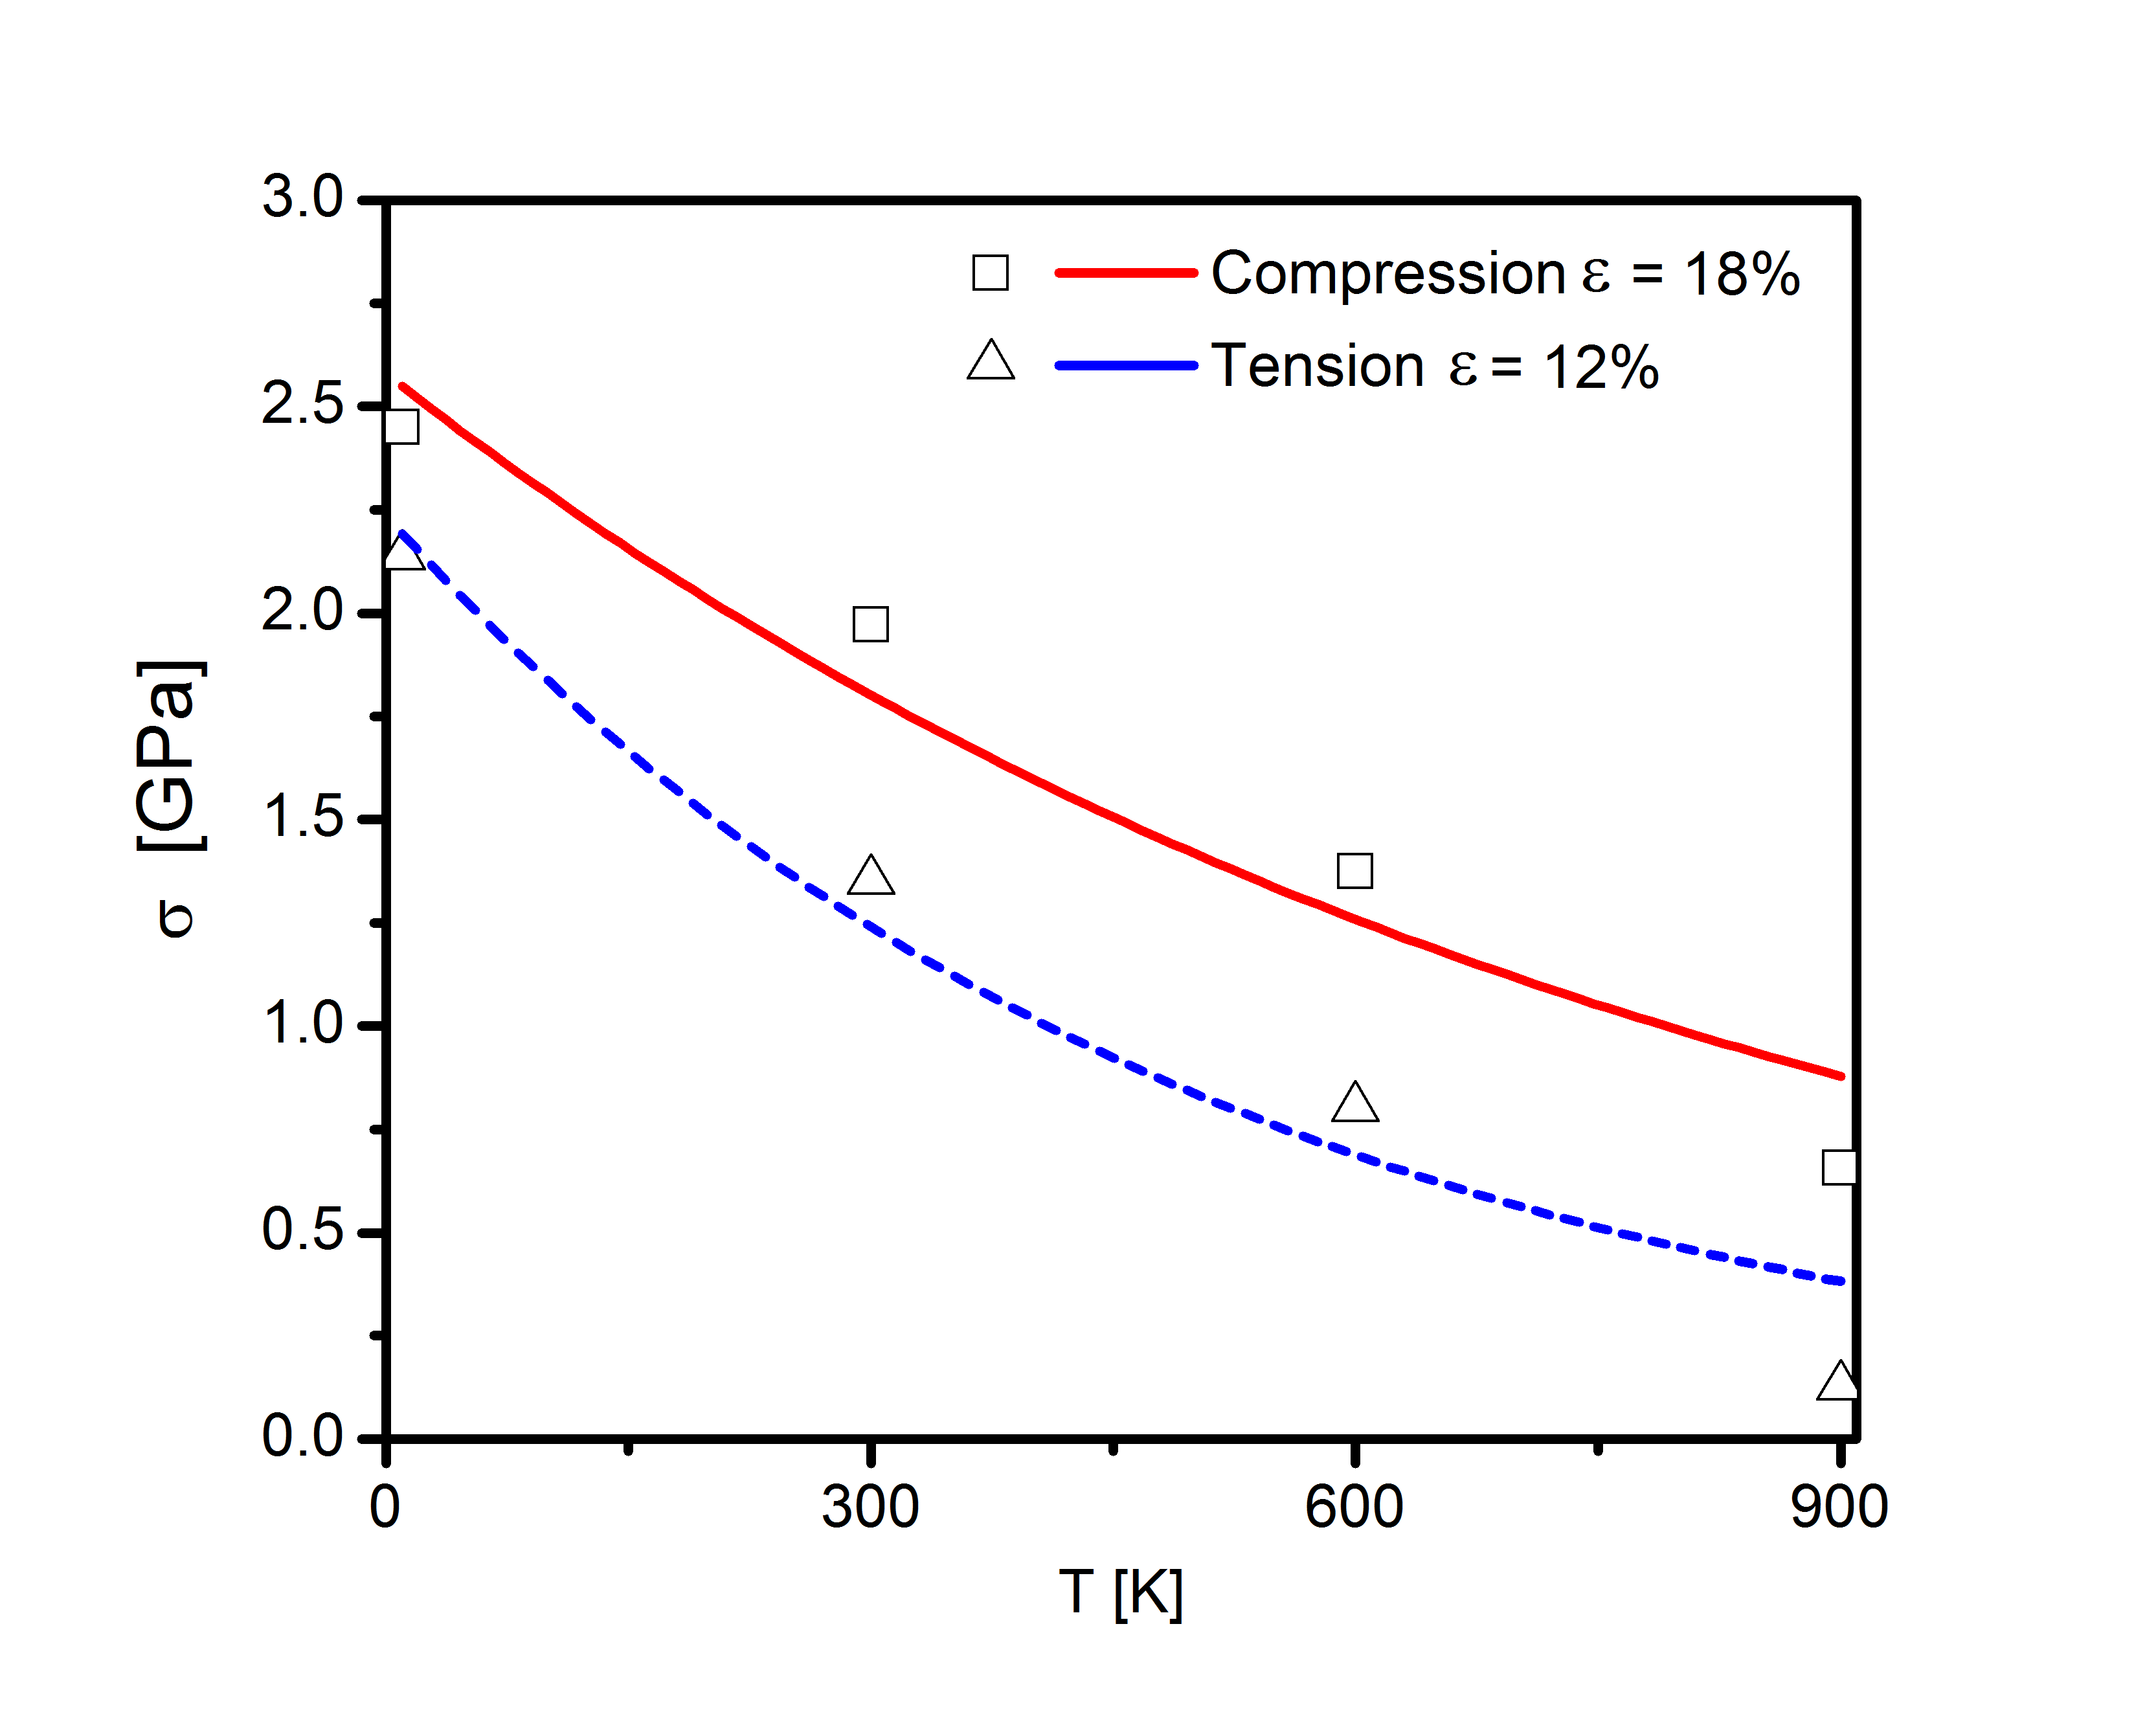
\includegraphics[width=10cm]{Cap_3/Fit1218.png}
\caption[Fit tensión de von Mises-temperatura.]{Fit tensión de von Mises-temperatura. En tracción se utilizaron tensiones a deformaciones más bajas para evitar las fluctuaciones debidas a la nucleacion del poro.}
\label{C3:fg:peakVMises1218VsT}
\end{figure} 

\cite{cheng11} buscó describir el comportamiento de una muestra sometida a esfuerzos cortantes puros al inicio de la plasticidad  como una funcion de algunas variables, incluyendo la temperatura, basándose en un CSM (modelo de corte cooperativo???). Sus cálculos dieron una dependencia de la temperatura de la forma $(T/T_g)^{2/3}$. Tratamos de comparar este comportamiento con nuestros resultados. Simplificando la expresión en \cite{cheng11}, obtuvimos la siguiente expresión:

%\cite{cheng11} attempted to describe the behavior of the onset of plasticity under pure shear, as a function of several variables, including temperature, based on a CSM (cooperative shear model). The resulting temperature dependence was (T/Tg)2/3, and we try to apply this behavior to our results. Simplifying the expression in \cite{cheng11}, we obtain the following expression:

\begin{eqnarray}
\frac{\sigma{}_{y}}{G} = A+B\left( \frac{T}{Tg} \right)^{2/3}
\label{C3:eq:onsetPlast}
\end{eqnarray}

donde $\sigma{}_{y}$ es la tensión de fluencia, mientras que A y B son parámetros que se deben ajustar. Para obtener la tensión de fluencia en nuestras simulaciones utilizamos la regla 0.2: asumimos que la plasticidad comienza cuando la curva esfuerzo-deformación se aleja un 20\% del comportamiento elástico, el cual lo extrapolamos a partir de puntos obtenidos a deformaciones muy bajas (menores a $\epsilon$=1\%). En las tablas \ref{C3:tb:initPropsTen}-\ref{C3:tb:initPropsComp} presentamos valores para los coeficientes de la ecuación \ref{C3:eq:onsetPlast} obtenidos para las curvas que se muestran en la figura \ref{C3:fg:fitDosTercios}. En esta figura comparamos las curvas ajustadas para tracción y compresión con el resultado de \cite{johnson05}, quien obtuvo, para  deformación cortante pura, la siguiente expresión:

%where $\sigma{}_{y}$ is the yielding stress, while A and B are parameters of the fit. To obtain the yield stress in our simulations we assume that plasticity starts when the stress-strain curve departs 20\% from the linear elastic behavior extrapolated from very low strains (below $\epsilon$=1\%). In Tables 2-3 we present the values for the coefficients of equation (2) obtained for the curves shown in Figure 6. In this figure we compare the fittings for tension and compression with the result from \cite{johnson05}, who obtained, for experiments under pure shear deformation the following expression:

\begin{eqnarray}
\frac{\tau _{y}}{G} = 0.036-0.016\left( \frac{T}{Tg} \right)^{0.62}
\label{C3:eq:johnsonSamwer}
\end{eqnarray}

donde $\tau _{y}$ es la tensión de fluencia cortante. Observamos que la ecuación \ref{C3:eq:onsetPlast} puede aproximar relativamente bien tanto la tracción como la compresión uniaxial. Hay ciertas discrepancias con la aproximación experimental de la ecuación \ref{C3:eq:johnsonSamwer}, pero notamos que los coeficientes de la aproximación tienen grandes márgenes de error, y los datos muestran mucha dispersión. Por ejemplo, el exponente es  0.62 $\pm$ 0.2.
	
%where $\tau _{y}$ is the shear yield strength .We observe that equation (2) fits both uniaxial tension and compression quite well. There are discrepancies with the experimental fit from equation (3), but we note that the coefficients in that fit had large error bars, and data showed large dispersion. For instance, the exponent was 0.62 $\pm$ 0.2.

\begin{figure}[htp]
\centering
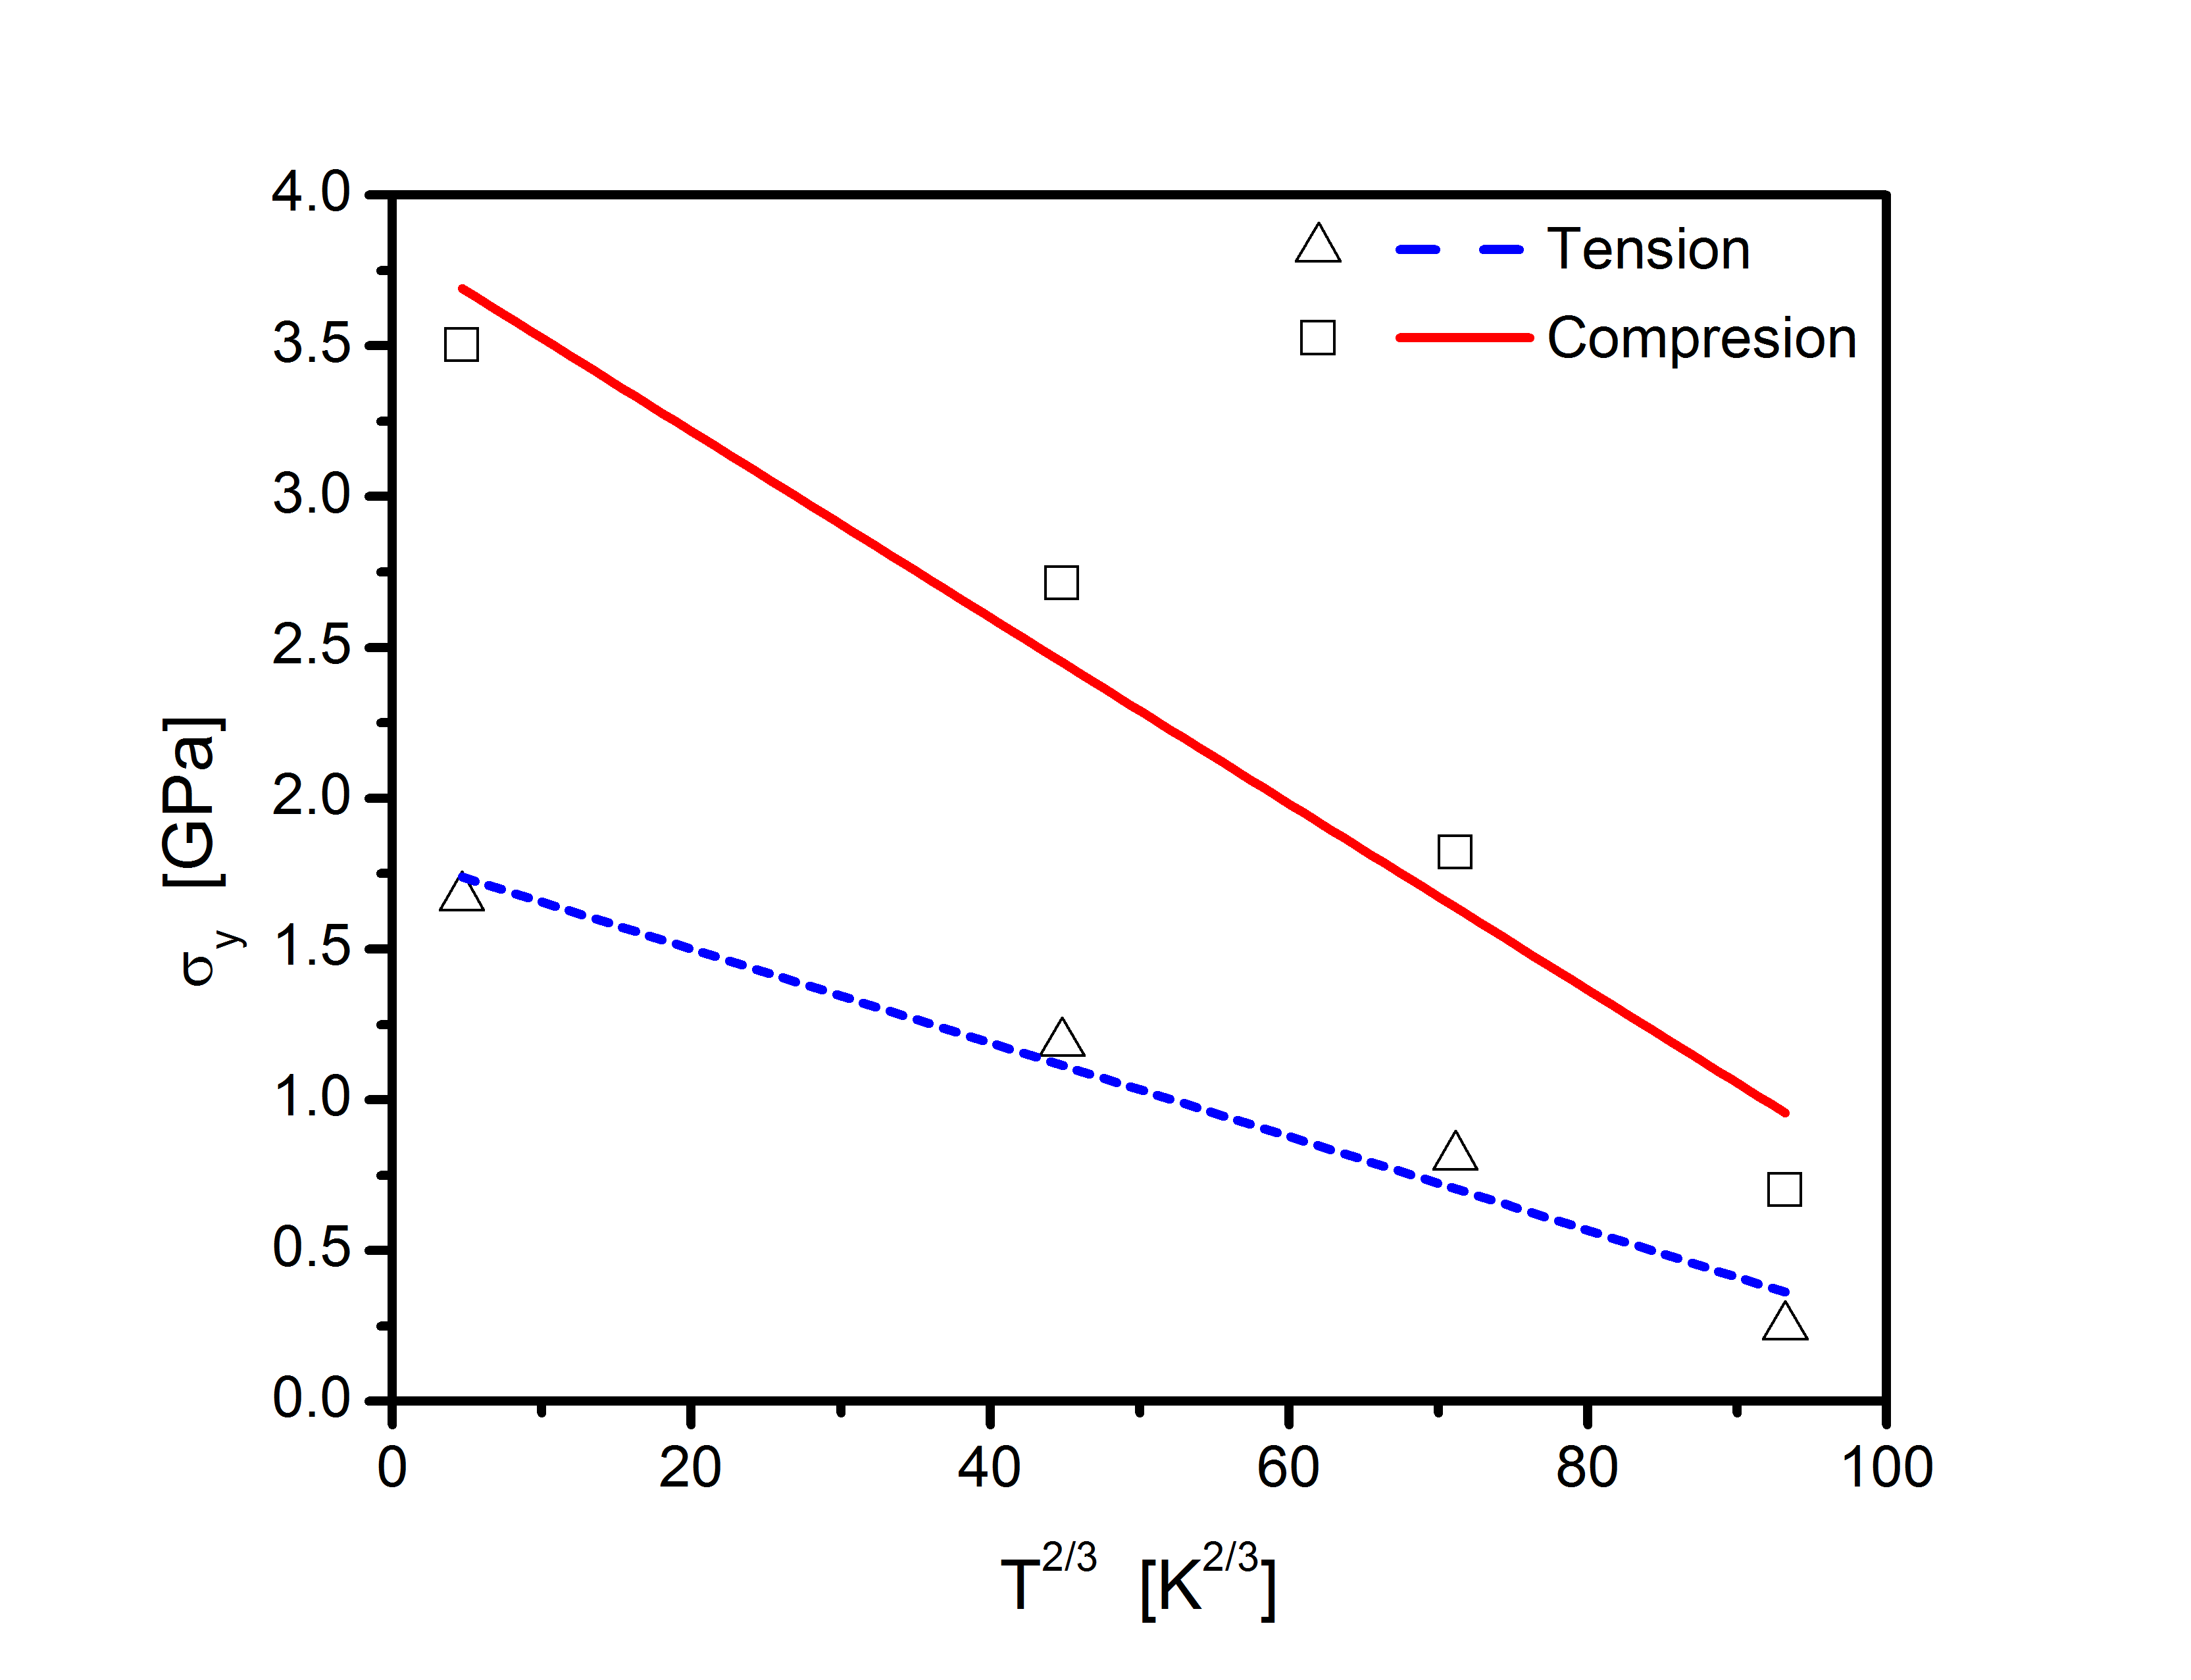
\includegraphics[width=10cm]{Cap_3/Fitdostercios.png}
\caption[Fit tensión de fluencia-temperatura.]{Fit tensión de fluencia-temperatura. Utilizamos los valores experimentales de $T_g$ y G (\cite{johnson05}) para normalizar nuestros resultados.}
\label{C3:fg:fitDosTercios}
\end{figure}

La figura \ref{C3:fg:sampleTen} muestra la tensión de von Mises atómica para la muestra completa (tracción a T=300K). A pesar de la evidencia de comportamiento plástico en las curvas esfuerzo-deformación, no observamos evidencia de bandas de corte.

%Figure 7 shows atomic von Mises stress for the complete sample in the case of tension at T=300K. Despite the evidence of plastic behavior in stress-strain curves, we do not observe evidence of shear bands.

De acuerdo a un estudio en nanocables de vidrio metalico (\cite{xiao12}), la presencia de bandas de corte depende fuertemente de la velocidad de enfriamiento del vidrio. En este caso, para las velocidades de enfriamiento utilizadas en la creación de nuestra muestra, no se deberian observar bandas de corte, como se observa en la figura \ref{C3:fg:sampleTen}. Sin embargo, en secciones posteriores (\ref{ss:BC}) se observarán trazos de bandas de corte graficando la deformación atómica en lugar del esfuerzo atomico.

%According to a recent study in metallic glass nanowires (\cite{xiao12}), the presence of shear bands strongly depends on the quenching rate of the glass. In this case, for the quenching rates used in the creation of our sample, shear bands should not be observed, as shown in Figure 7.

\begin{figure}[htp]
\centering
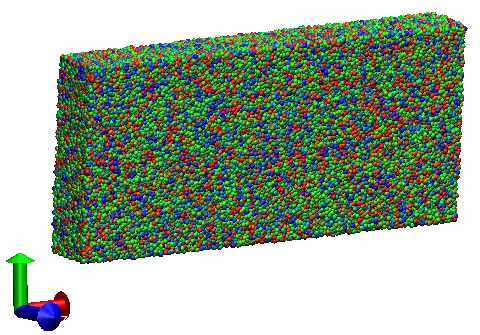
\includegraphics[width=10cm]{Cap_3/All_300K_6pstrain_sacale100-280_Trac.png}
\caption[Vista de la muestra a $\epsilon$=6\%, bajo tracción uniaxial, a T=300 K.]{Vista de la muestra a $\epsilon$=6\%, bajo tracción uniaxial, a T=300 K. Los colores representan la tensión de von Mises, siendo el color rojo para esfuerzos grandes y el color azul para esfuerzos pequeños, en una escala RGB. El rango de esfuerzos varia de 100 GPa a 280 GPa. No se observan SB. La visualización fue realizada con VMD \citep{humphrey96}. Resultados similares se observan a otras temperaturas simuladas.}
\label{C3:fg:sampleTen}
\end{figure}

Cuando deformamos el vidrio metálico mediante compresión uniaxial podemos observar un comportamiento similar de las curvas esfuerzo-deformación mostradas en la figura \ref{C3:fg:sStrainComp} con respecto a las curvas de tracción mostradas en la figura \ref{C3:fg:sStrainTen}, siempre a deformaciones menores al 15\%. Luego del 15\% deformación las curvas de compresión tienen una forma suave debido a que no hay nucleación de poros.

%When the metallic glass deforms under uniaxial compression we can observe a similar behavior in the stress-strain curves shown in Figure 1 (b) to the curves corresponding to tension in Figure 1 (a), for strains below 15\%. However, since there is no void nucleation above 15\%, the behavior of the curves is smooth even at very high strains.

Las figuras \ref{C3:fg:youngVsT}-\ref{C3:fg:fitDosTercios} muestran las mismas aproximaciones que las usadas para tracción. Las aproximaciones también son razonables, incluso con una ecuación de aproximación simple como la mostrada en la ecuación \ref{C3:eq:thermalFit}.

%Figures 3-6 show the same type of fit that the one used for tension, and there is also a reasonable adjustment, even with the simple functional form shown in equation (1).

La figura \ref{C3:fg:sampleComp} muestra que, de igual manera que en la muestra bajo tracción, no se observan bandas de corte.

%Figure 8 shows that, similarly to the sample under tension, no shear bands are observed, as expected given the high quenching rate of the glass used here.

\begin{figure}[htp]
\centering
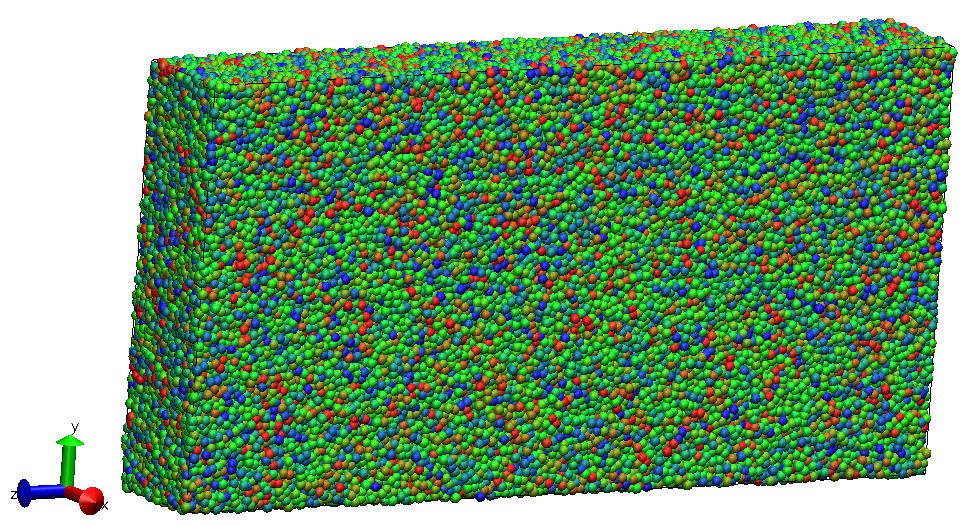
\includegraphics[width=10cm]{Cap_3/All_300K_6pstrain_sacale100-400_Comp.png}
\caption[Vista de la muestra a $\epsilon$=6\%, bajo compresión uniaxial, a T=300 K.]{Vista de la muestra a $\epsilon$=6\%, bajo compresión uniaxial, a T=300 K. Los colores representan la tensión de von Mises, siendo el color rojo para esfuerzos grandes y el color azul para esfuerzos pequeños, en una escala RGB. El rango de esfuerzos varia de 100 GPa a 400 GPa. No se observan SB. La visualización fue realizada con VMD \citep{humphrey96}. Resultados similares se observan a otras temperaturas simuladas.}
\label{C3:fg:sampleComp}
\end{figure}

\subsection{Bandas de corte}
\label{ss:BC}

Como se mencionó previamente, es posible observar bandas de corte graficando la deformación atómica de la muestra. Para esto se utiliza la herramienta Ovito, la cual utiliza el procedimiento descripto en \cite{shimizu07} para calcular la deformación atómica. La figura \ref{C3:fg:SBs} muestra el resultado.

\begin{figure}[htp]
\centering
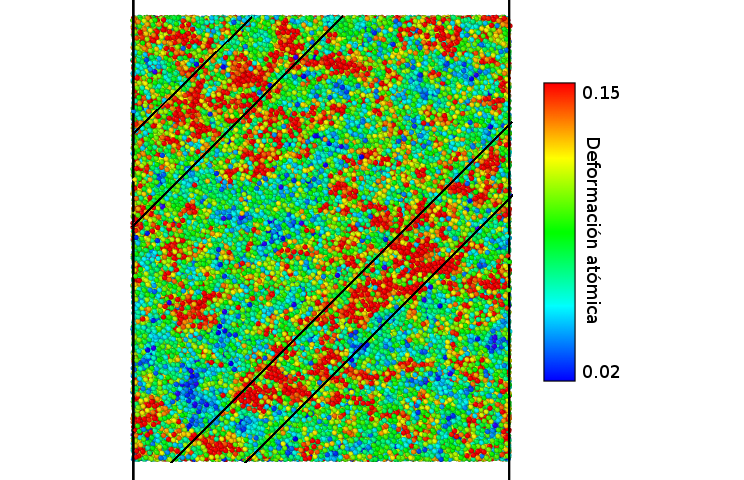
\includegraphics[width=10cm]{Cap_3/ShearBand.png}
\caption[Corte de la muestra a $\epsilon$=14\%, bajo compresión uniaxial, a T=300 K.]{Corte de la muestra a $\epsilon$=14\%, bajo compresión uniaxial, a T=300 K. Los colores representan la deformación atómica, siendo el color rojo grandes deformaciones y el color azul pequeñas deformaciones, en una escala RGB. El rango de deformación varia de 0.02 a 0.15. La visualización fue realizada con Ovito \citep{stukowski10}. Se eliminan los efectos de la deformación homogénea para poder apreciar mejor la deformación heterogénea producto de las bandas de corte.}
\label{C3:fg:SBs}
\end{figure}

Es posible apreciar que las bandas de corte se forman con una dirección predominantemente diagonal, a prácticamente $45º$. Las bandas de corte representan deformación heterogénea, lo cual puede llevar a la falla frágil del material. Esto es algo importante a tener en cuenta ya que puede reducir considerablemente la vida útil del material. En capítulos subsiguientes trataremos algunos métodos para retardar la propagación de bandas de corte.

\subsection{Simulación de la muestra con condiciones de frontera libres.}

Para verificar la dependencia con las condiciones de borde, se realizaron simulaciones con condiciones de frontera laterales libres, como se muestra en la figura \ref{C3:fg:libres}. Bajo tracción hay una pequeña disminución de la sección transversal de la muestra, como era de esperar. Esto puede ser observado en la figura \ref{C3:fg:cross}. Tambien podemos observar que la forma de la sección transversal cambia de rectangular a elíptica, debido a un efecto de minimización de la energía de superficie.

%To verify that the absence of shear bands is not due to periodic conditions during deformation, simulations were carried out with free lateral boundary conditions, as shown in Figure 10. Under tension there is a slight decrease in the cross section of the sample, as expected. This is shown in Figure 11. We can also observe that the shape of the cross section has changed from rectangular to elliptical, due to surface energy minimization.

Estas simulaciones son similares a aquellas realizadas sobre nanocables de vidrio metálico en \cite{xiao12}. Bajo compresión, se observa pandeo. En ninguno de los casos se observan bandas de corte.

%These simulations are similar to those of metallic glass nanowires seen in \cite{xiao12}. Under compression, buckling is observed. In both cases there is a lack of shear bands, as expected with the cooling rates used in our samples.

\begin{figure}[htp]
\centering
\subfloat[Tracción]{
	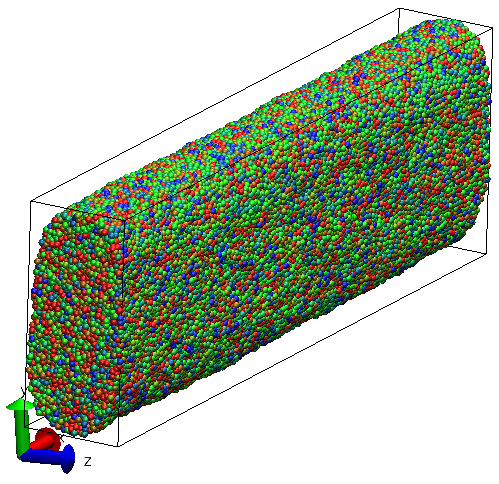
\includegraphics[width=8cm]{Cap_3/900libresTen.png}
	\label{C3:fg:libresTen}}
\subfloat[Compresión]{
	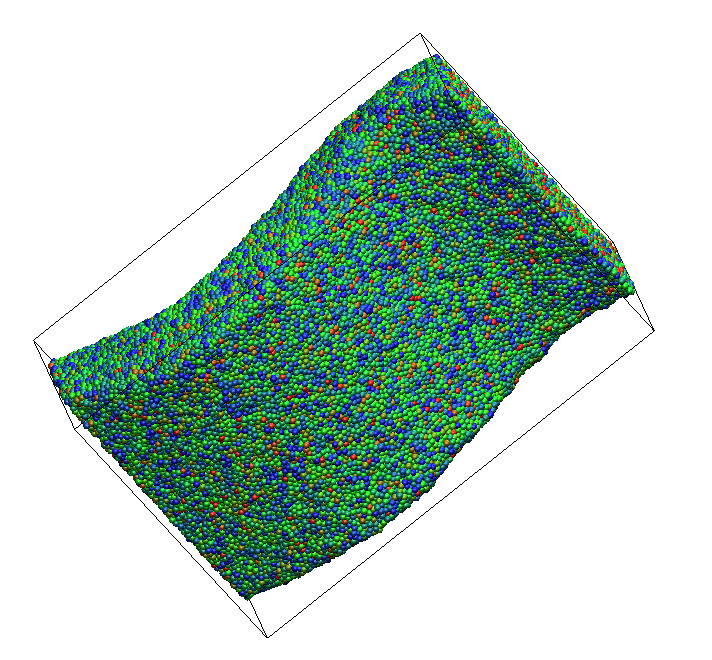
\includegraphics[width=8cm]{Cap_3/300libresComp.png}
	\label{C3:fg:libresComp}}
\caption[Simulaciones a tracción y compresión usando condiciones de frontera libres.]{Simulaciones a tracción y compresión usando condiciones de frontera libres. En ambos casos $\epsilon$=0.20. En la muestra a tracción, T=900K, y T=300K a compresión. No se observa estricción en el caso a tracción, posiblemente debido a que la simulación se realizó a una temperatura superior a $T_g$.}
\label{C3:fg:libres}
\end{figure}

\begin{figure}[htp]
\centering
\subfloat[]{
	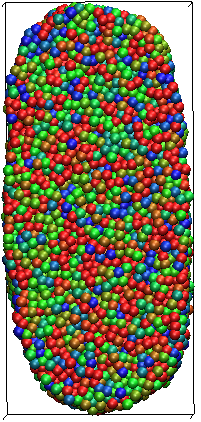
\includegraphics[width=3cm]{Cap_3/crossa.png}
	\label{C3:fg:crossExtreme}}
\subfloat[]{
	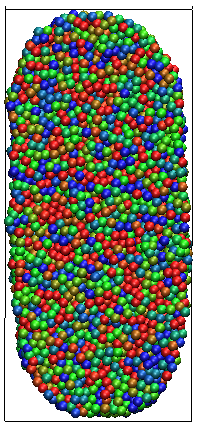
\includegraphics[width=3cm]{Cap_3/crossb.png}
	\label{C3:fg:crossMiddle}}
\caption[Sección transversal a diferentes distancias sobre el eje z, para la simulación presentada en la figura \ref{C3:fg:libres}]{Sección transversal a diferentes distancias sobre el eje z, para la simulación presentada en la figura \ref{C3:fg:libres}. (a) Sección próxima al extremo. (b) Sección central de la muestra. No se aprecia estricción, incluso a altas deformaciones.}
\label{C3:fg:cross}
\end{figure}

\section{Conclusiones}


%Atomistic simulations of bulk metallic glasses (BMGs) mechanical behavior under tension and compression were performed using molecular dynamics (MD) simulations. The increase of sample temperature produces a considerable decrease of the samples elastic modulus. The same applies to maximum von Mises stress. It is observed that the elastic modules are practically the same under tension or compression at different temperatures, but the maximum stress in compression is much higher. The behavior with temperature can be adjusted reasonably well with an exponential decay with temperature, typical of thermal activated phenomena.

%No shear bands are observed, which is to be expected given that our glass was generated with very high quenching rates. Since no shear bands are observed in our simulations, the identification of plasticity is complex. Surely there are shear areas, "shear transformation zones" (STZ), composed of a few atoms that experience high shear stresses. The identification of these areas requires a very detailed observation of the sample, involving much longer simulations than those used here. An alternative to study plasticity is the examination of Voronoi polyhedra, which can help to identify these areas. Such studies are in progress.

%In the future, using more powerful computational resources than available for this work, we plan to create samples with quenching rates orders of magnitude slower, with the aim to observe the possible formation of shear bands.

%A detailed understanding of the influence of temperature, quenching rates, etc., in the mechanical properties of metallic glasses will allow obtaining necessary properties for their application in new technologies, including applications under extreme conditions, such as aerospace missions or materials in nuclear reactors. Studies like the one presented here will contribute to this understanding and accelerate novel material development. 